\documentclass{beamer}
\usetheme{Boadilla}
\usepackage{minted}
\usepackage{hyperref}
\usepackage{tikz}
\usetikzlibrary{shapes,positioning}
\usepackage{graphicx}
\usepackage{fontawesome}
\usepackage{fancyvrb}
\usepackage{adjustbox}
\usepackage{multicol}
\usepackage{subfig}
\usepackage{xcolor}
\usepackage{optparams}
\usepackage{xstring}
\usepackage[
    backend=biber, 
    natbib=true,
    style=numeric,
    sorting=none,
    style=verbose-ibid,
]{biblatex}
\addbibresource{citations.bib}
\usepackage{pgfpages}
\definecolor{ao(english)}{rgb}{0.0, 0.5, 0.0}
\definecolor{burgundy}{rgb}{0.5, 0.0, 0.13}
\setbeameroption{show notes}
\setbeameroption{show notes on second screen=right}
%\setbeameroption{hide notes}

\newlength{\mintednumbersep}
\AtBeginDocument{%
  \sbox0{\tiny00}%
  \setlength\mintednumbersep{8pt}%
  \addtolength\mintednumbersep{-\wd0}%
}

\def\footshortciteintern[#1][#2]#3{%
\ifx#1\empty 
% Nur Autor
\footnote{\citeauthor{#3}, \citeyear{#3}.}
\else
\ifx#2\empty
% Autor und Seite
\footnote{\citeauthor{#3}, \citeyear{#3}, #1.}
\else
% Autor, Seite und vgl.
\expandafter  
\footnote{\citeauthor{#3}, \citetitle{#3}, \citeyear{#3}, \citeurl{#3}.}
\fi
\fi
}
\newcommand*\footshortcite{%
\optparams{\footshortciteintern}{[\empty][\empty]}
}
\newcommand*\footmediumcite{%
\optparams{\footshortciteintern}{[][]}
}

\title[TF representations for music separation]{Time-Frequency Representations for Music Source Separation}
\subtitle{Final project presentation}
\author{Sevag Hanssian}
\date{April 22, 2021}
\institute{MUMT 622, Winter 2021}
\setbeamertemplate{navigation symbols}{}

\begin{document}

\begin{frame}
\maketitle
\end{frame}

\begin{frame}
	\frametitle{Music Source Separation}
	Musical sources are often categorized as either predominantly harmonic, predominantly percussive, or as singing voice.\footfullcite{musicsepgood} In this project, I consider both cases (HPSS and harmonic/percussive/vocal)
	\begin{figure}
		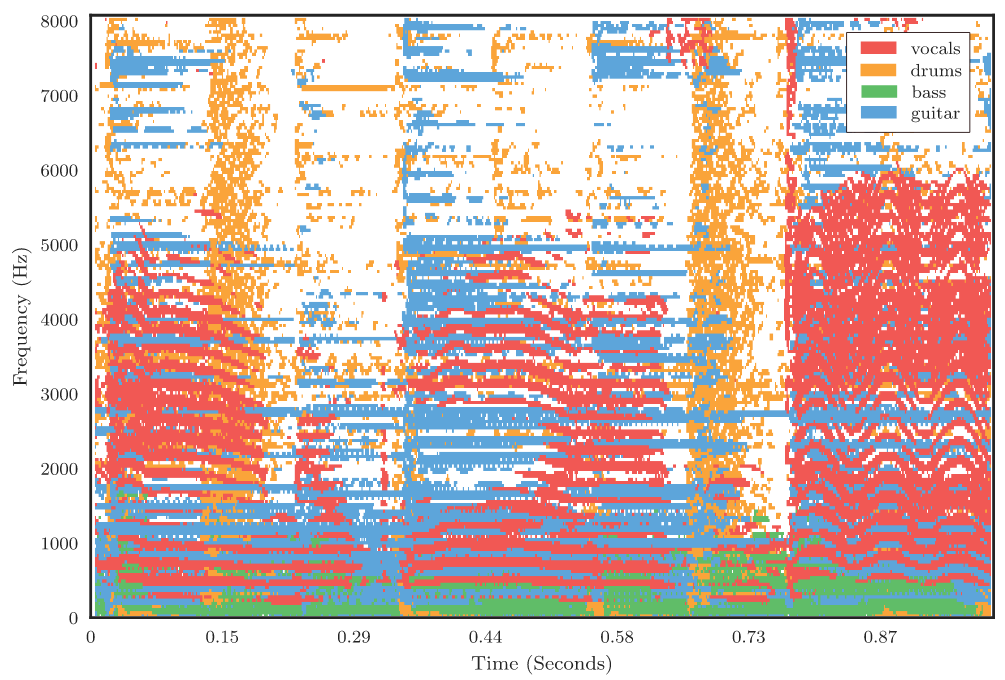
\includegraphics[width=7cm]{./mss1.png}
		\caption{Typical music sources in a mix}
	\end{figure}
\end{frame}

\note{
	\begin{itemize}
		\item
			steady-state/transient
		\item
			tonal/transient in ltfat world
	\end{itemize}
}

\begin{frame}
	\frametitle{Music Source Separation}
	A notable property of musical sources is that they are typically \textit{sparse} in the sense that for the majority of points in time and frequency, the sources have very little energy present\footshortcite{musicsepgood}
	\begin{figure}
		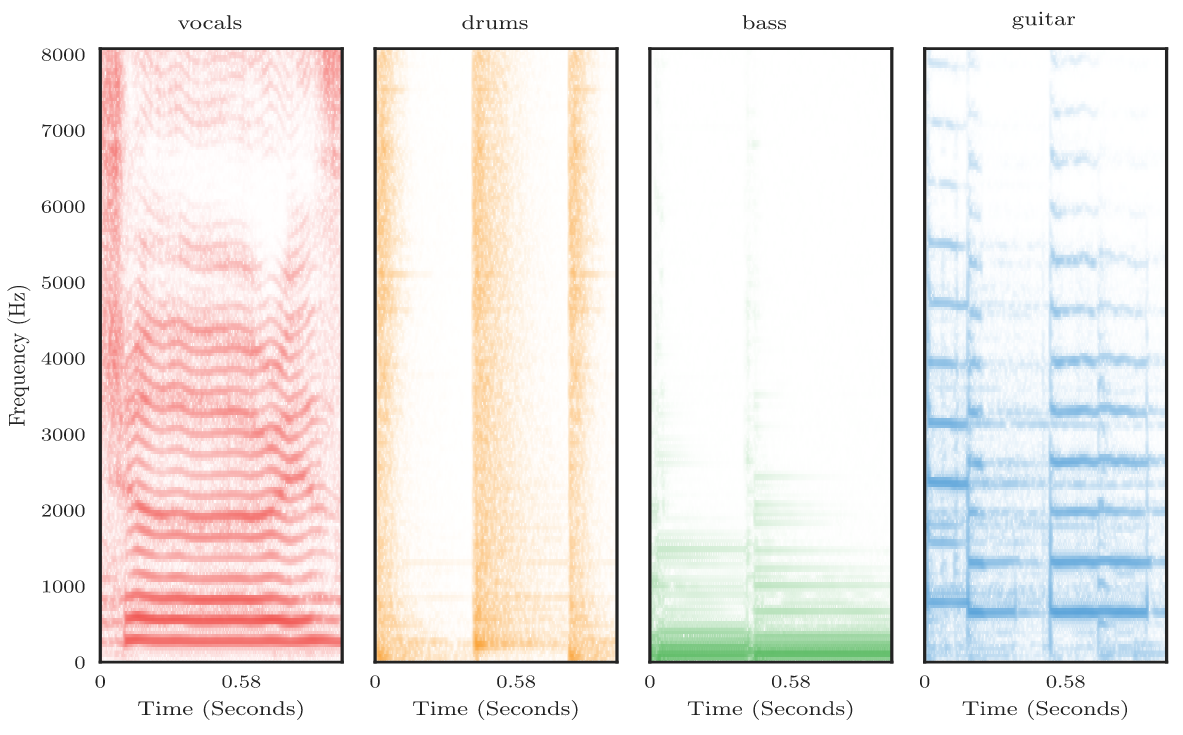
\includegraphics[width=8cm]{./mss2.png}
		\caption{Typical music sources, separated}
	\end{figure}
\end{frame}

\begin{frame}
	\frametitle{Music Source Separation}
	\begin{figure}
		\subfloat[Mixing block diagram]{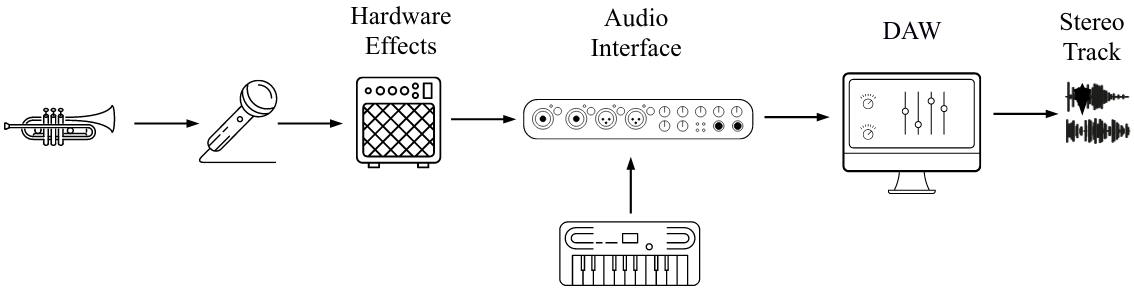
\includegraphics[width=10cm]{./mss3.png}}\\
		\vspace{0.1em}
		\subfloat[Unmixing block diagram]{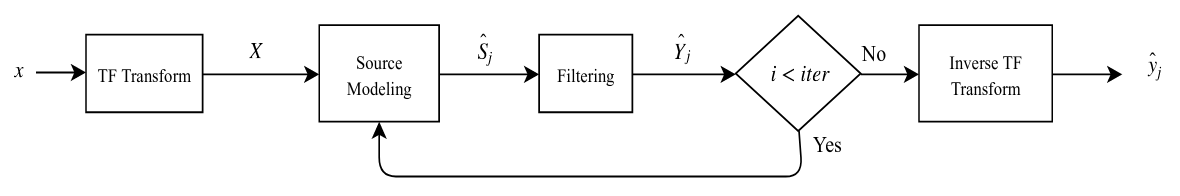
\includegraphics[width=10cm]{./mss4.png}}
		\caption{Typical block diagrams for source mixing and source separation (aka ``unmixing'')\footshortcite{musicsepgood}}
	\end{figure}
\end{frame}

\begin{frame}
	\frametitle{Median filtering HPSS}
	Form of Kernel Additive Model -- describe harmonic sounds as horizontal, percussive sounds as vertical, and apply median filters on magnitude spectrogram to estimate each\footfullcite{fitzgerald1}
	\begin{figure}[ht]
		\vspace{-0.75em}
		\subfloat[Anticausal/offline]{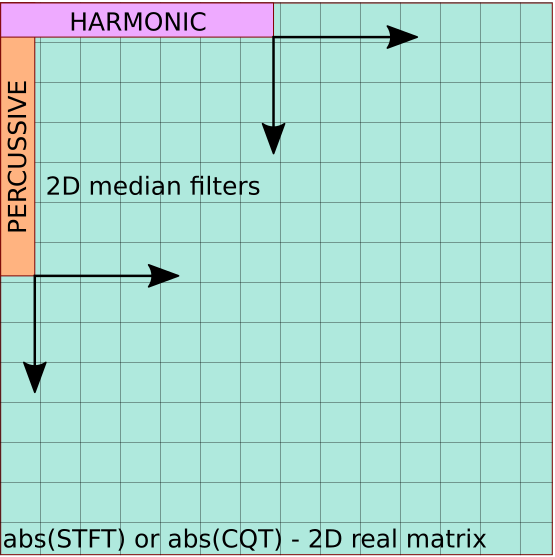
\includegraphics[height=3.5cm]{./singlemfilt.png}}
		\hspace{0.2em}
		\subfloat[Causal/realtime]{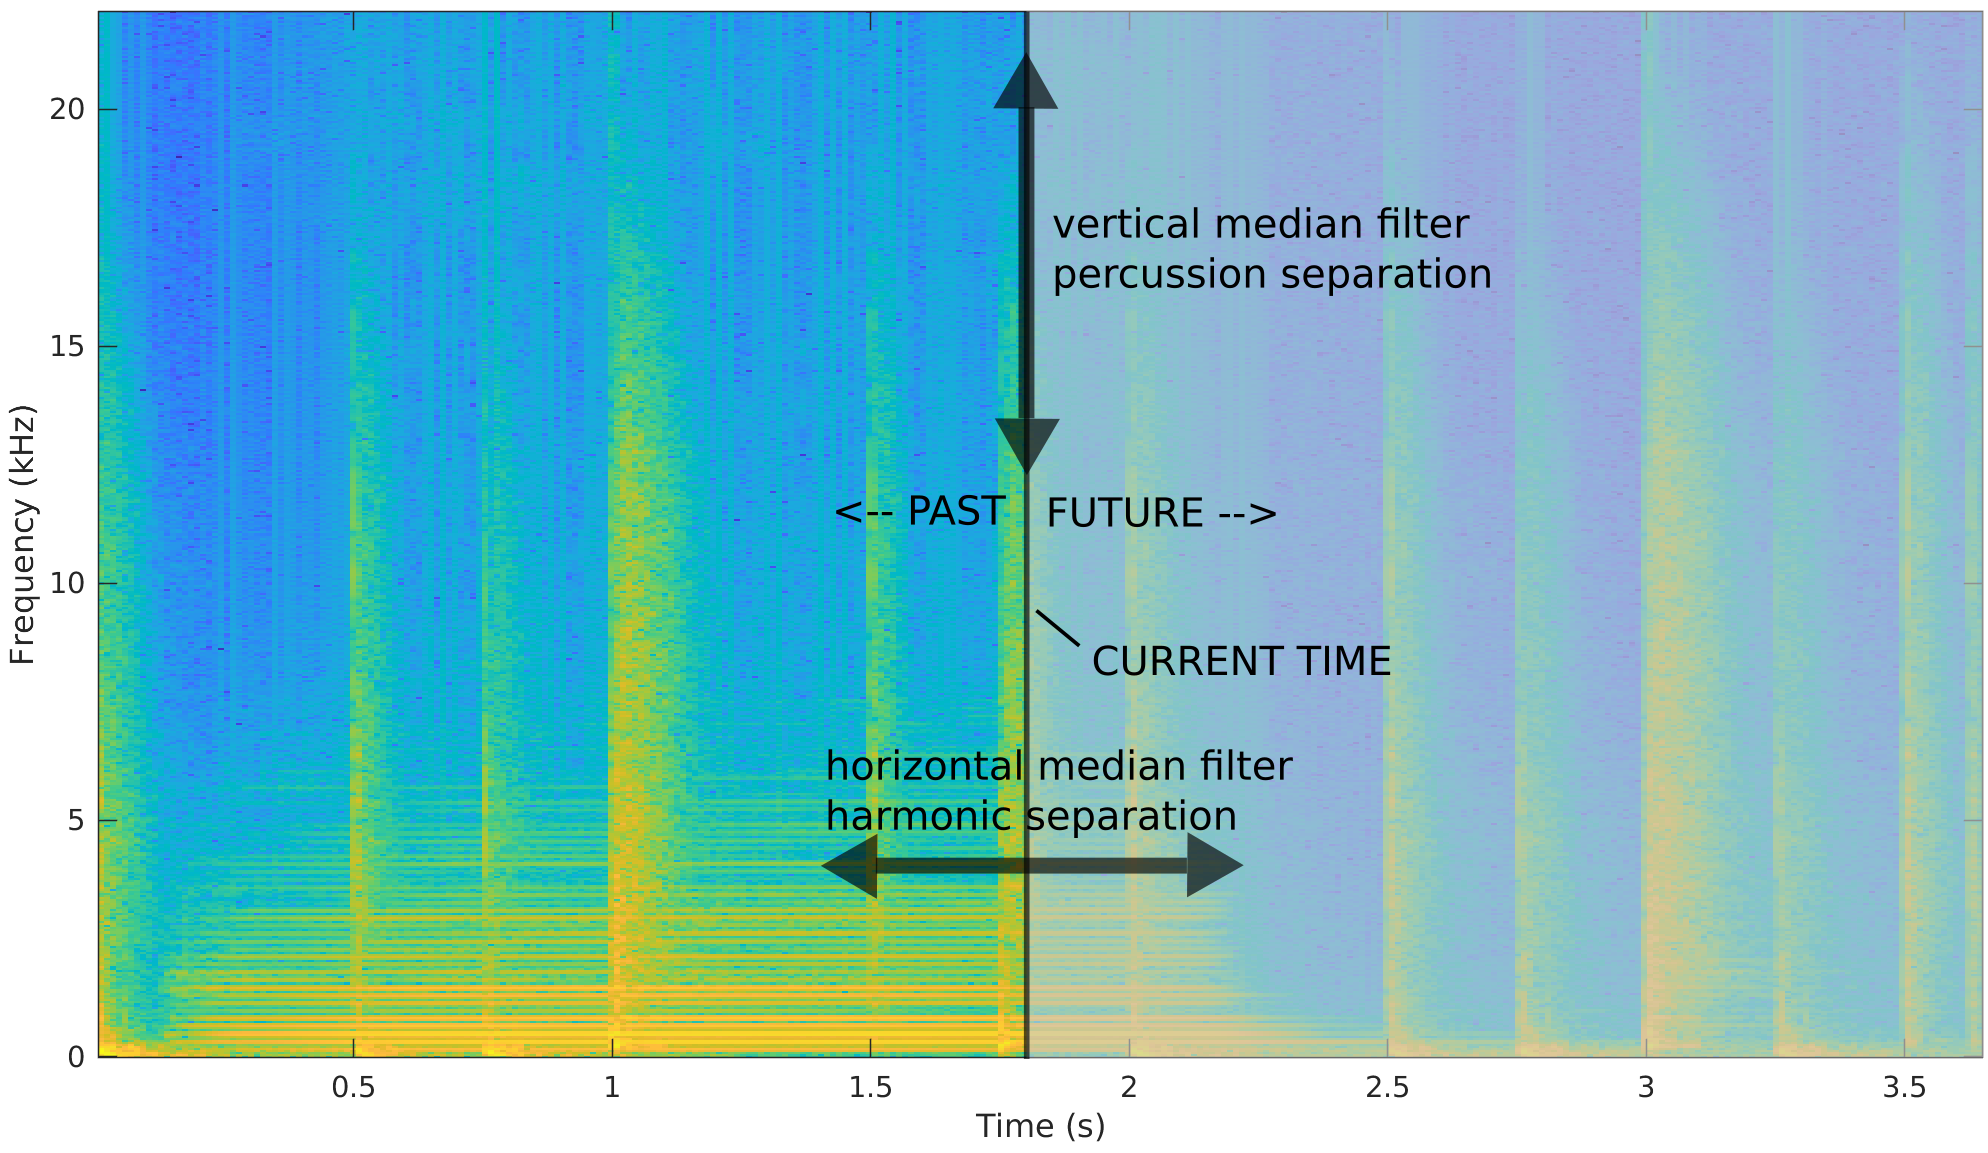
\includegraphics[height=3.5cm]{./rthpss_causality.png}}
		\caption{Median filter on STFT, anticausal and causal cases}
	\end{figure}
\end{frame}

\note{
	\begin{itemize}
		\item
			sliding STFT, perform causal median filtering, then invert
		\item
			keep several columns of STFT in memory, perform windowing + overlap-add -- presented this in 501
	\end{itemize}
}

\begin{frame}
	\frametitle{Median filtering HPSS}
	Use harmonic and percussive magnitude spectrogram estimates to compute soft masks\footshortcite{fitzgerald1} or hard masks:\footfullcite{driedger}
	\begin{figure}[ht]
		\vspace{-1em}
		\subfloat[Mixed signal]{{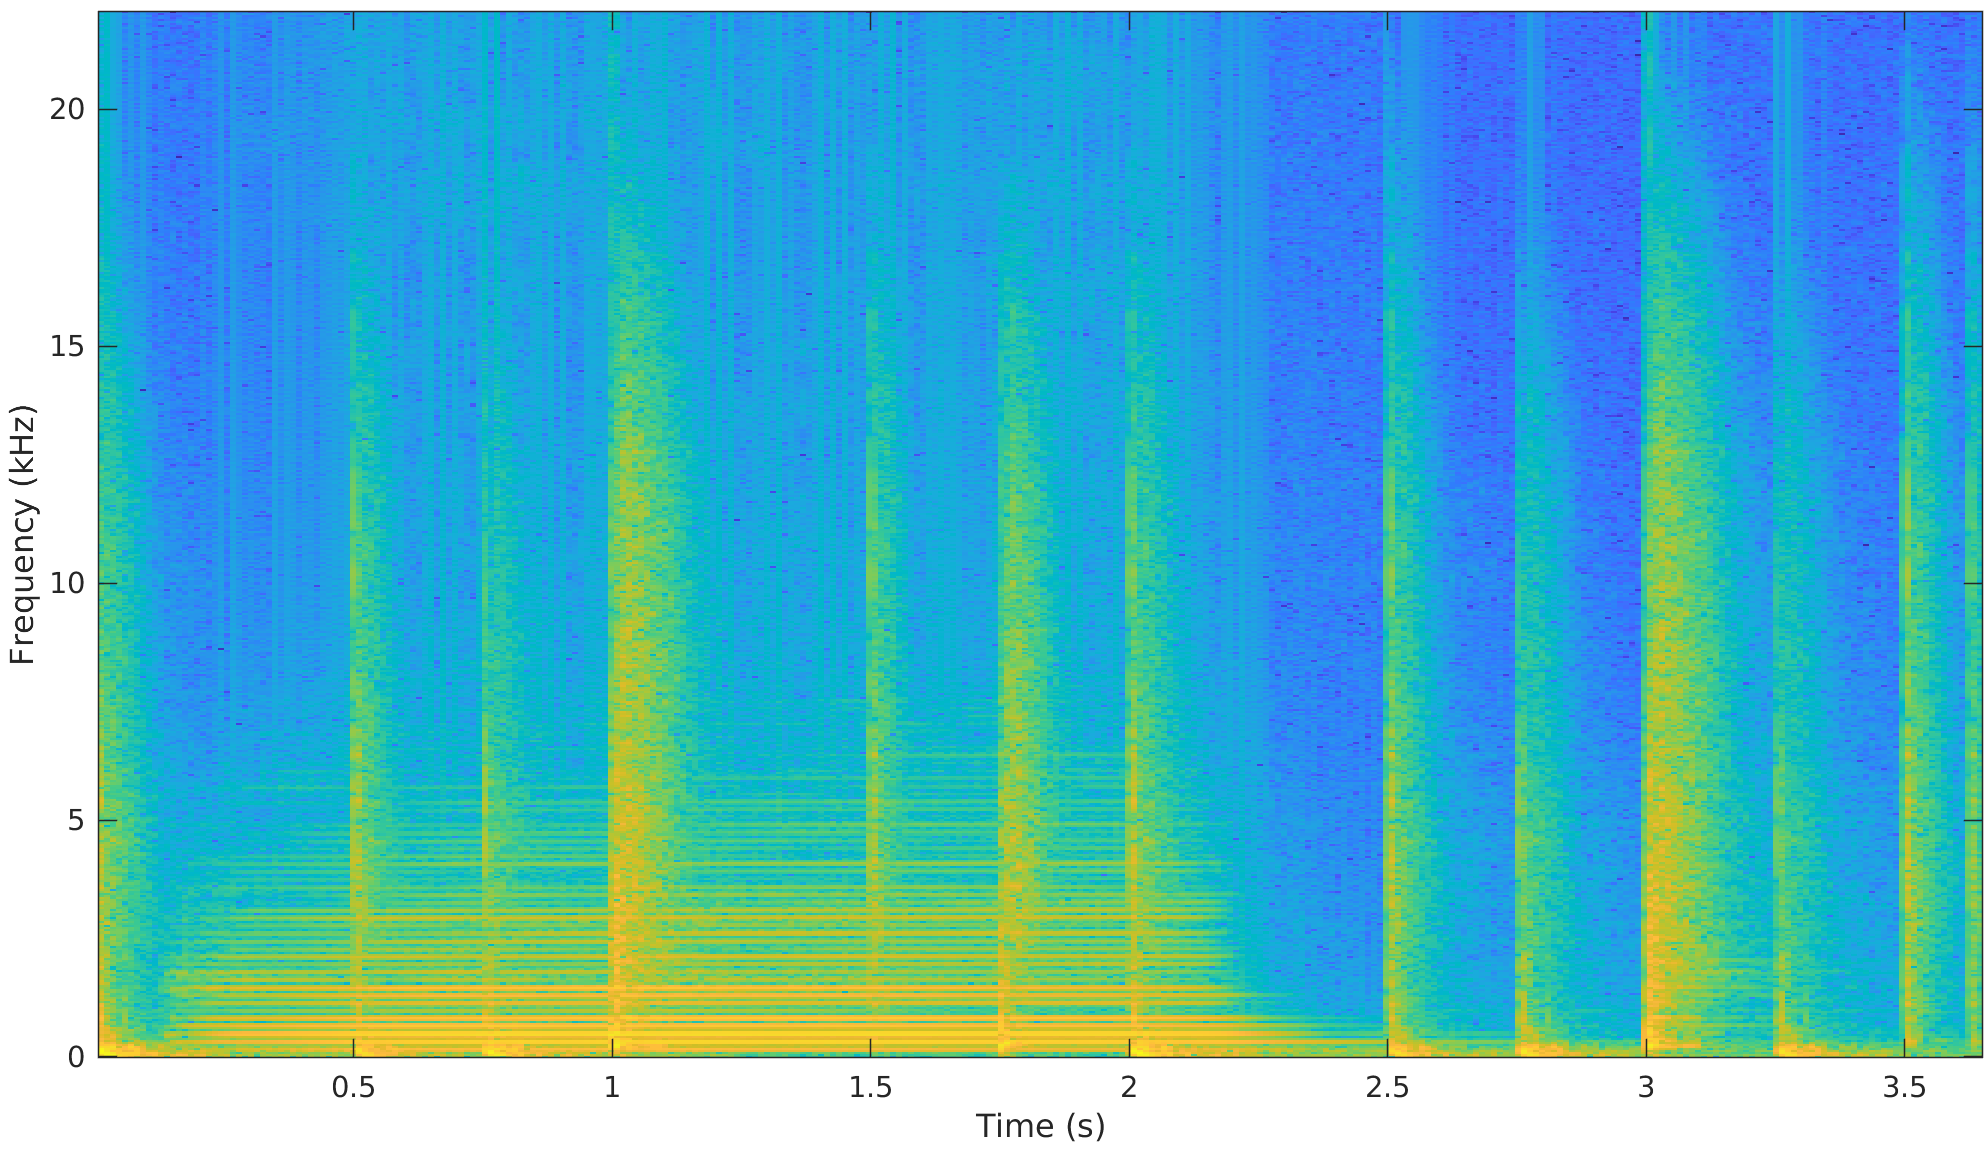
\includegraphics[width=3.9cm]{./mixedspecgram.png} }}
		\subfloat[Percussive separation]{{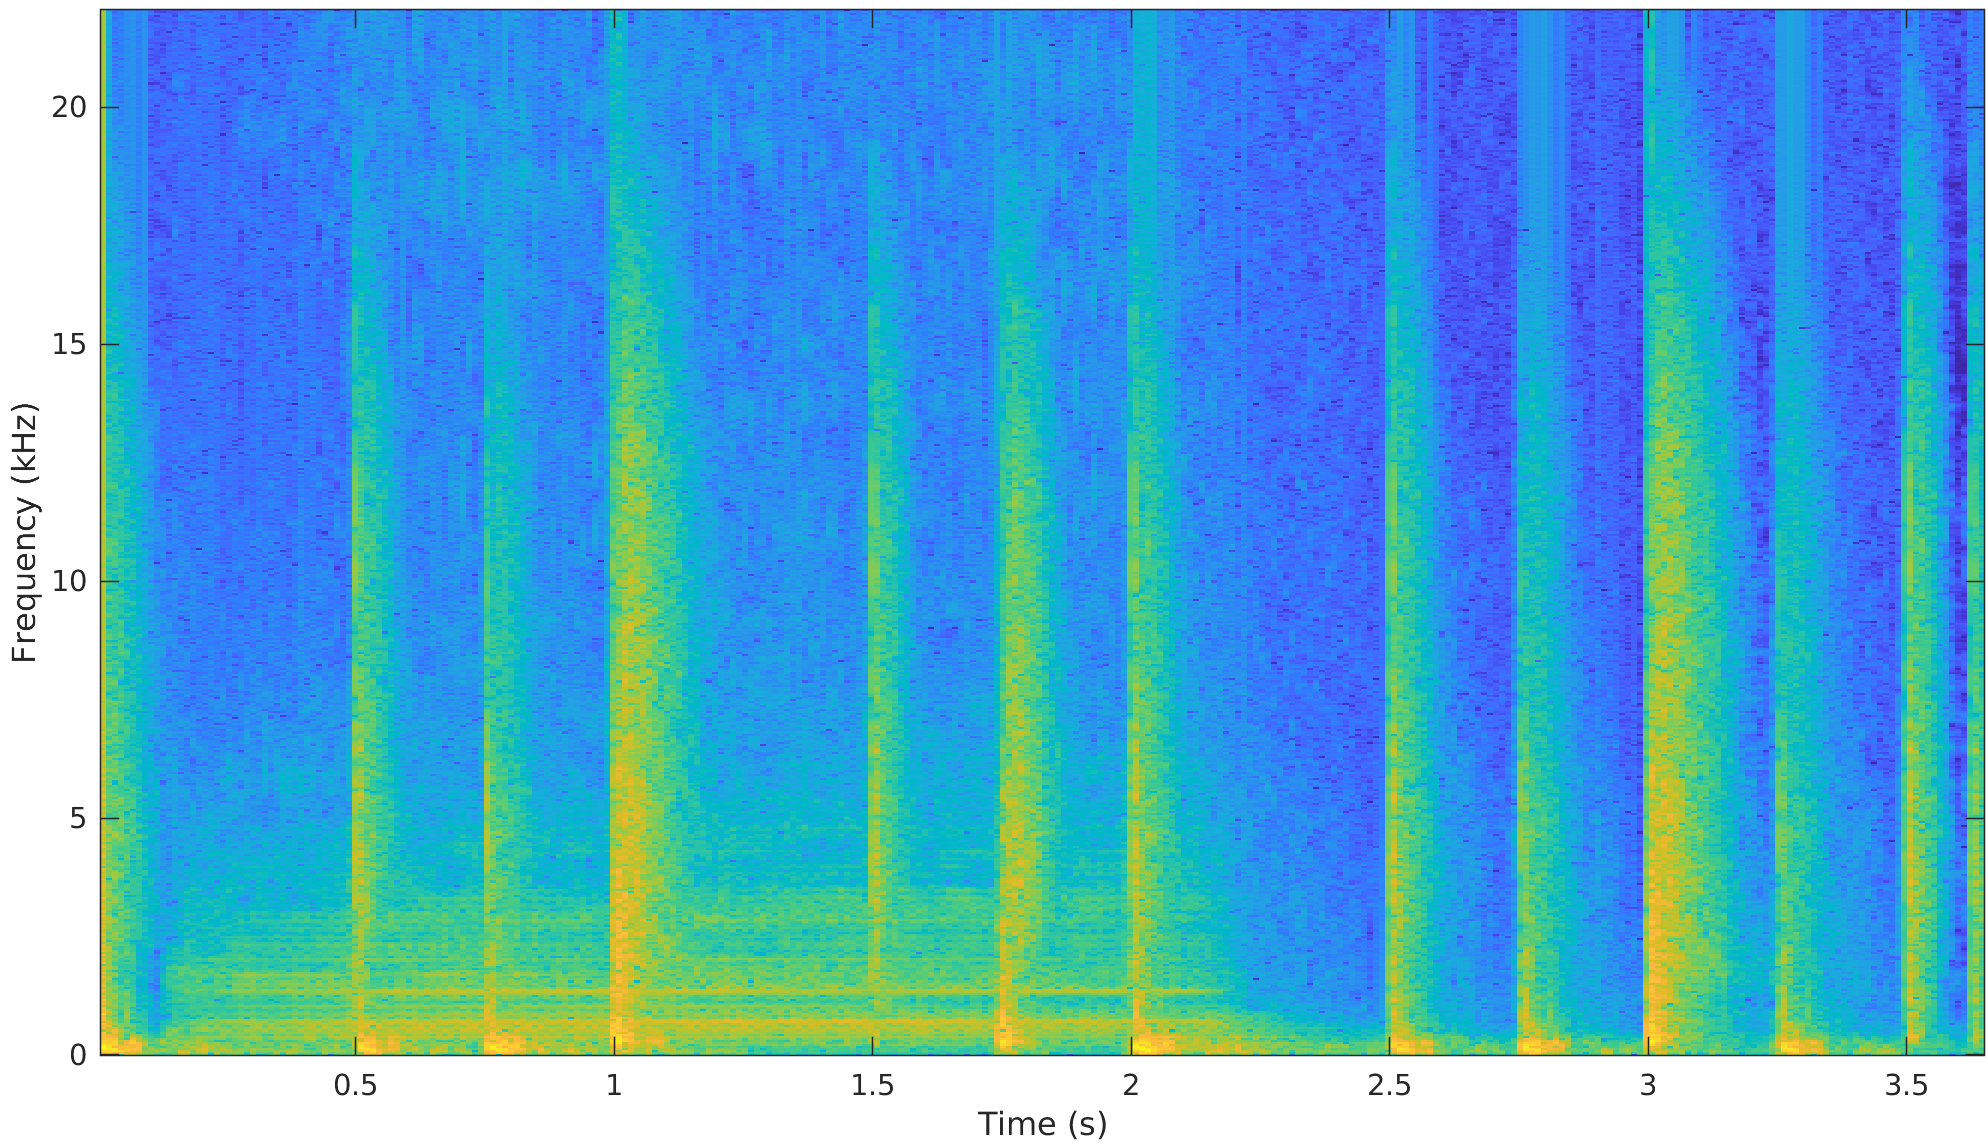
\includegraphics[width=3.9cm]{./perc_soft.png} }}
		\subfloat[Harmonic separation]{{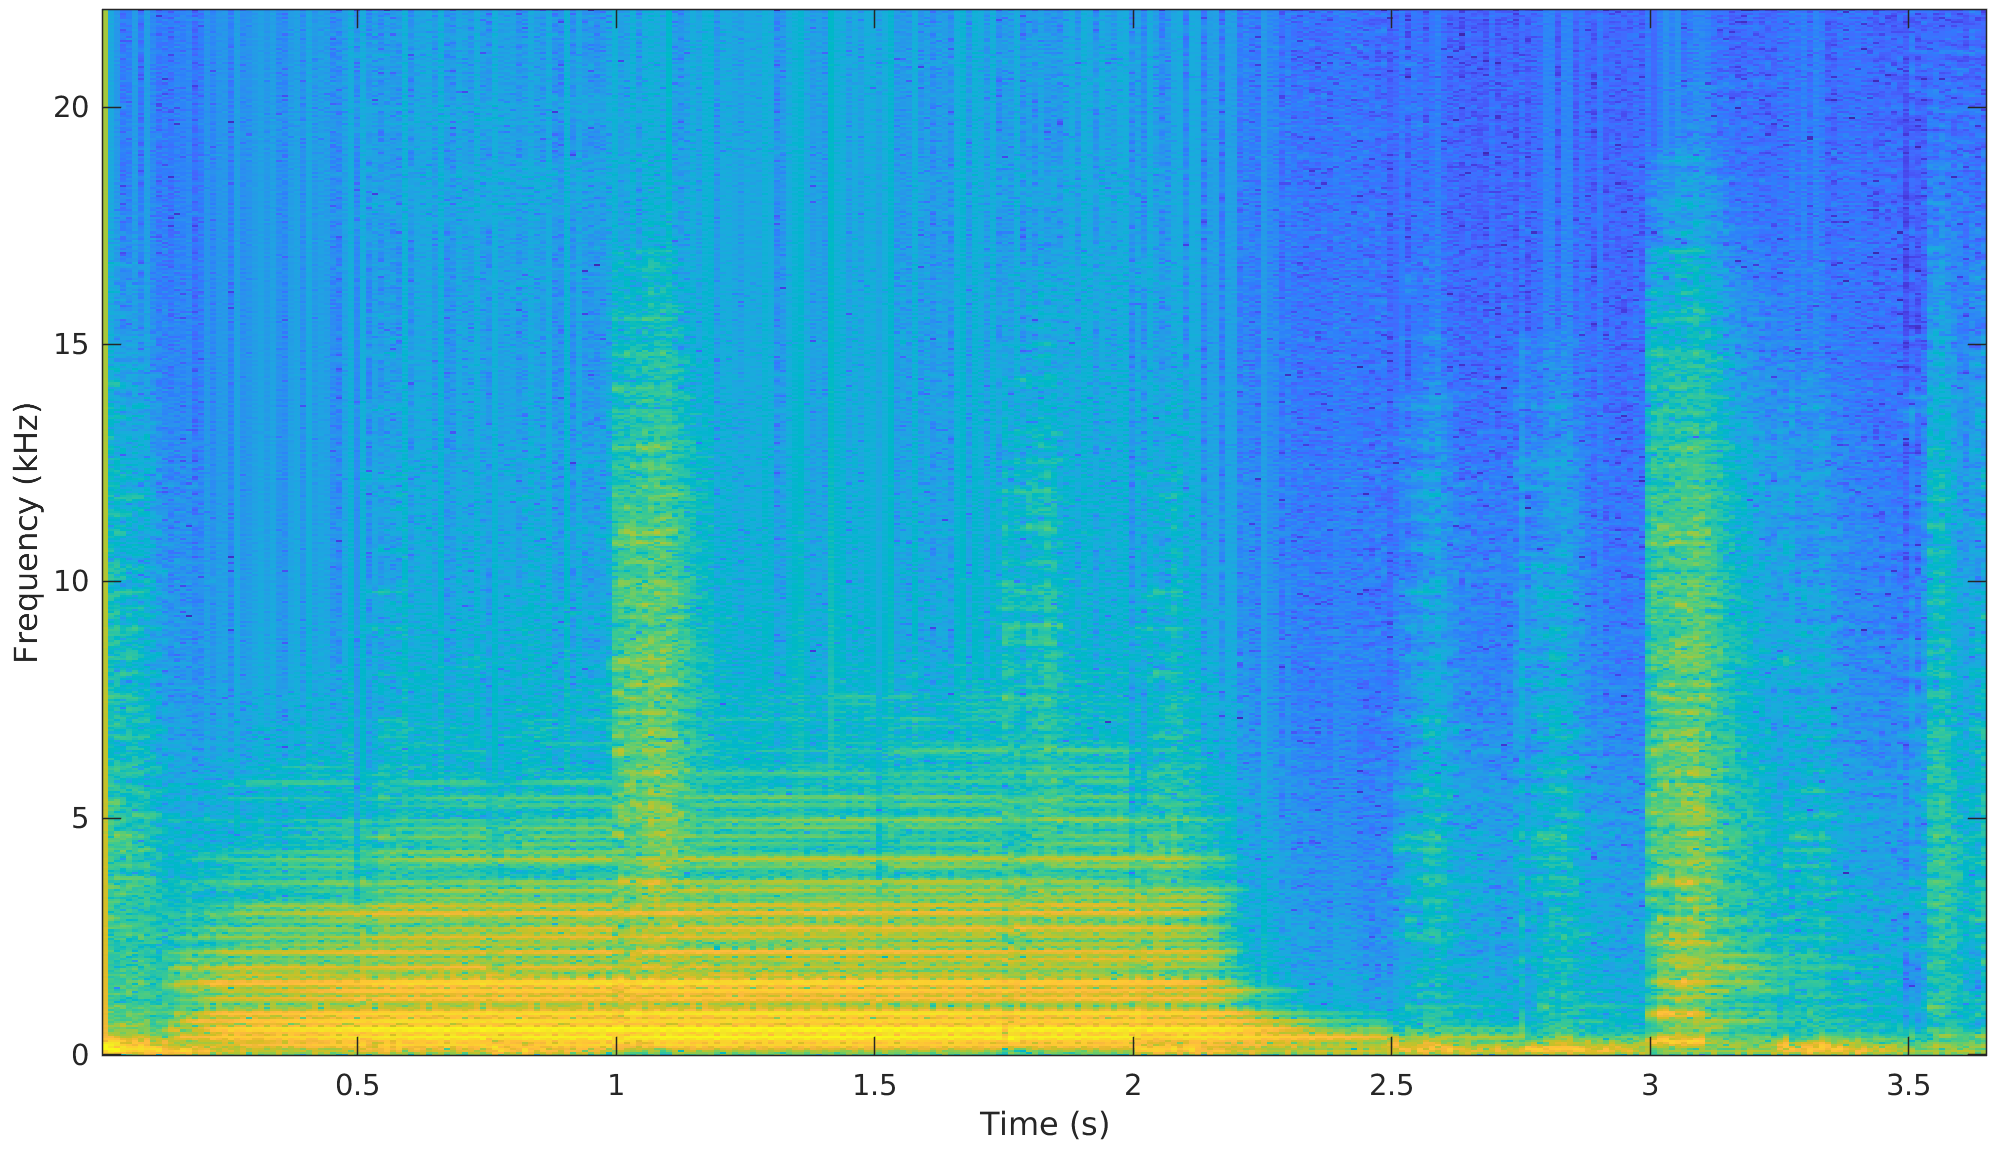
\includegraphics[width=3.9cm]{./harm_soft.png} }}
		\caption{Example of median filtering HPSS}
		\vspace{-1em}
	\end{figure}
	Originally based on STFT spectrogram. CQT works fine too.
\end{frame}

\begin{frame}
	\frametitle{Median filtering HPSS}
	Soft mask, Wiener filter:\footshortcite{fitzgerald1}
	\[ M_{\text{harmonic}} = \frac{|\hat{S}_{\text{harmonic}}|^{2}}{|\hat{S}_{\text{harmonic}}|^{2} + |\hat{S}_{\text{percussive}}|^{2}} \]
	Hard mask, binary mask:\footshortcite{driedger}
	\[ M_{\text{harmonic}} = \frac{|\hat{S}_{\text{percussive}}|}{|\hat{S}_{\text{harmonic}}| + \epsilon} > \beta \]
	Setting $\beta > 1.0$ leads to a third residual component:
	\[ M_{\text{residual}} = 1 - (M_{\text{harmonic}} + M_{\text{percussive}}) \]
	Soft mask gives higher audio quality\footshortcite{masking}
\end{frame}

\note{
	\begin{itemize}
		\item
			define how different harmonic and percussive should be
	\end{itemize}
}

\begin{frame}
	\frametitle{Iterative median filtering HPSS}
	2-pass HPSS,\footshortcite{driedger}, harmonic/percussive/vocal:\footshortcite{fitzgerald2}
	\begin{figure}[ht]
		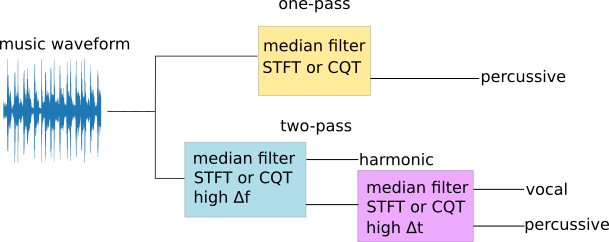
\includegraphics[width=8cm]{./medianfiltdiagram.png}
		\caption{One- or two-pass median filter HPSS}
	\end{figure}
\end{frame}

\begin{frame}[fragile]
	\frametitle{HPSS MATLAB pseudocode}
\begin{figure}[h]
  \centering
 \begin{minipage}{0.48\textwidth}
  \centering
\begin{minted}[numbersep=\mintednumbersep,linenos,mathescape=true,breaklines,frame=single,escapeinside=||]{text}
|$s = \text{mixed audio}$|
|$\hat{S} = \text{STFT}(s)\text{\textbf{ or CQT}}$|
|$S = \text{abs}(\hat{S})$|
|$H = \text{medianfilter}(S, l_{H}, \text{axis}=2)$|
|$P = \text{medianfilter}(S, l_{P}, \text{axis}=1)$|
|$\text{\textbf{soft} } M_{H} = \frac{H^{p}}{H^{p} + P^{p}}, M_{P} = \frac{P^{p}}{H^{p} + P^{p}}$|
|$\text{\textbf{hard} } M_{H} = \frac{H}{P + \epsilon} \ge \beta, M_{P} = \frac{P}{H + \epsilon} > \beta$|
|$\hat{H} = \hat{S} \cdot M_{H}$|
|$\hat{P} = \hat{S} \cdot M_{P}$|
|$h = \text{ISTFT}(\hat{H})\text{\textbf{ or ICQT}}$|
|$p = \text{ISTFT}(\hat{P})\text{\textbf{  or ICQT}}$|
\end{minted}
 \end{minipage}
\hspace{0.02\textwidth}
 \begin{minipage}{0.48\textwidth}
  \centering
\begin{minted}[numbersep=\mintednumbersep,linenos,mathescape=true,breaklines,frame=single,escapeinside=||]{text}
|$s = \text{mixed audio}$|
|$\hat{S1} = \text{STFT}(s)\text{\textbf{ or CQT}}$|
|$ \text{1-pass algorithm } \rightarrow \hat{H1}, \hat{P1} $|
|$\text{\textbf{final harmonic} } h1 = \text{ISTFT}(\hat{H1})\text{\textbf{ or ICQT}}$|
|$p1 = \text{ISTFT}(\hat{P1})\text{\textbf{ or ICQT}}$|
|$\hat{S2} = \text{STFT}(p1)\text{\textbf{ or CQT}}$|
|$ \text{1-pass algorithm } \rightarrow \hat{H2}, \hat{P2} $|
|$h2 = \text{ISTFT}(\hat{H2})\text{\textbf{ or ICQT}}$|
|$\text{\textbf{final percussive} } p1 = \text{ISTFT}(\hat{P2})\text{\textbf{ or ICQT}}$|
\end{minted}
 \end{minipage}
  \captionof{listing}{1- and 2-pass median filtering HPSS algorithms}
\end{figure}
\end{frame}

\begin{frame}
	\frametitle{STFT, CQT, and TF resolution}
	STFT vs. CQT\footnote{\url{https://www.mathworks.com/help/wavelet/ref/cqt.html}} (based on NSGT\footmediumcite{balazs}):
	\begin{figure}[ht]
		\vspace{-0.6em}
		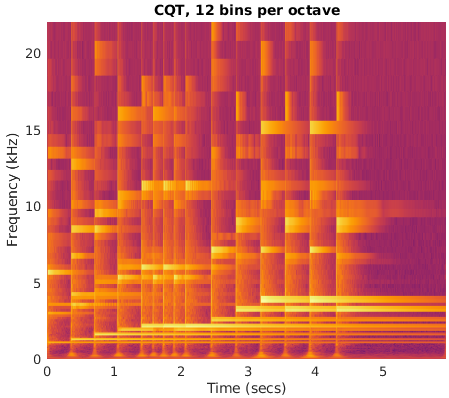
\includegraphics[width=3.5cm]{./glock_cqt12.png}
		\hspace{0.1em}
		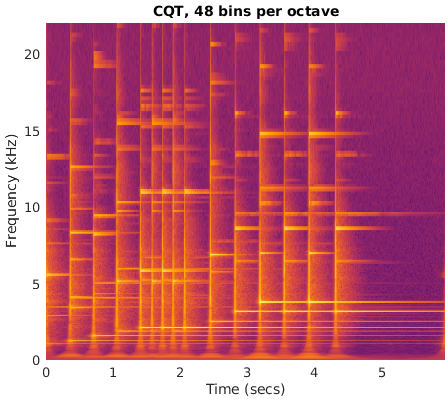
\includegraphics[width=3.5cm]{./glock_cqt48.png}\\
		\vspace{0.1em}
		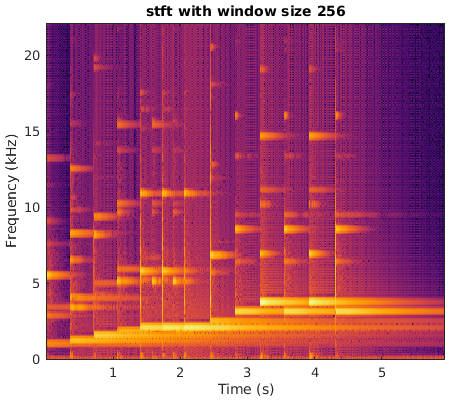
\includegraphics[width=3.5cm]{./glock_stft256.png}
		\hspace{0.1em}
		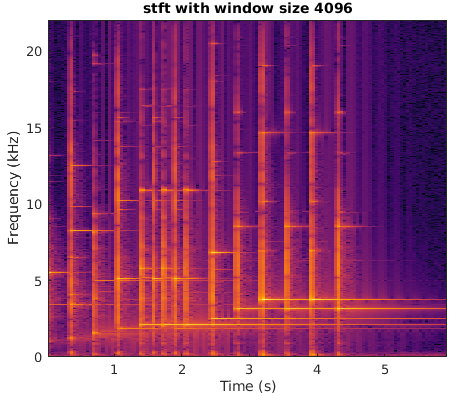
\includegraphics[width=3.5cm]{./glock_stft4096.png}
	\end{figure}
\end{frame}

\note{
	\begin{itemize}
		\item
			glockenspiel = default file of ltfat, the canonical sound for tonal/transient
		\item
			loaded by gspi function
		\item
			look how good the cqt is -- original motivation for this project, can we take the simple median filter algorithm and make it better with a better tf representation
	\end{itemize}
}

\begin{frame}
	\frametitle{Sparsity, entropy, and two window sizes}
	Sparsity and entropy are complementary concepts:\footfullcite{honeine2014entropy, pastor2015mathematics}
	\begin{itemize}
		\item
			\textit{Sparsity} is the property of concentrating most of the energy of $x$ in few coefficients of $w$
		\item
			\textit{Entropy} is the property of not concentrating most of the probability mass in few atoms of $p$ -- in other words, the entropy of a random variable is a concept of information theory that characterizes the unpredictability inherent in its outcomes
	\end{itemize}
	In every algorithm shown, the common element is a 2 dictionary wide + narrow window analysis, to represent tonal and transient parts of the input signal sparsely -- or, to represent tonal and transient parts of the input signal with low entropy/high significance
\end{frame}

\begin{frame}
	\frametitle{Structured sparsity}
	Group-LASSO:\footfullcite{sparsitykowalski} Lasso shrinkage (aka linear least squares regression\footmediumcite{tibshirani}\footmediumcite{dictionary2}) to the transform coefficients in the time and frequency dimensions
	\begin{figure}[ht]
		\vspace{-1em}
		\subfloat{\makebox[0.4\textwidth]{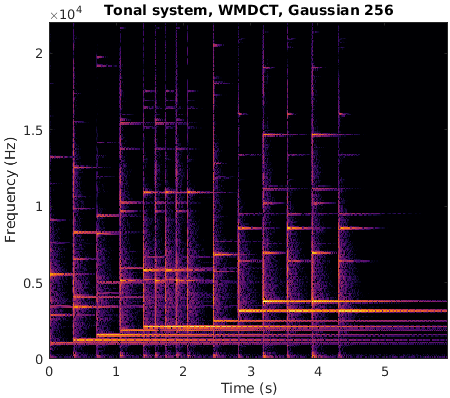
\includegraphics[height=3.5cm]{./glock_wmdct_tonal.png}}}
		\subfloat{\makebox[0.4\textwidth]{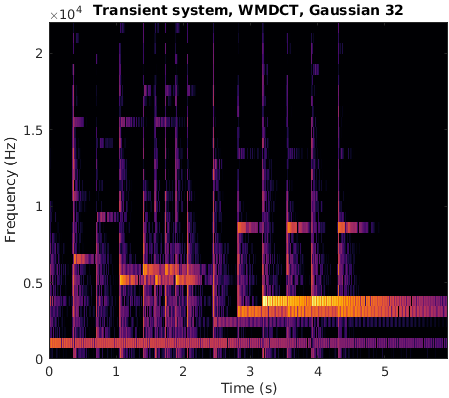
\includegraphics[height=3.5cm]{./glock_wmdct_transient.png}}}
		\caption{WMDCT frames for structured sparsity tonal/transient separation}
	\end{figure}
\end{frame}

\begin{frame}
	\frametitle{Structured sparsity}
	WMDCT\footfullcite{wmdct} + Group-LASSO -- ``audioshrink''\footnote{\url{https://homepage.univie.ac.at/monika.doerfler/StrucAudio.html}, \url{https://ltfat.github.io/doc/demos/demo_audioshrink.html}}
	\begin{figure}[ht]
		\vspace{-0.5em}
		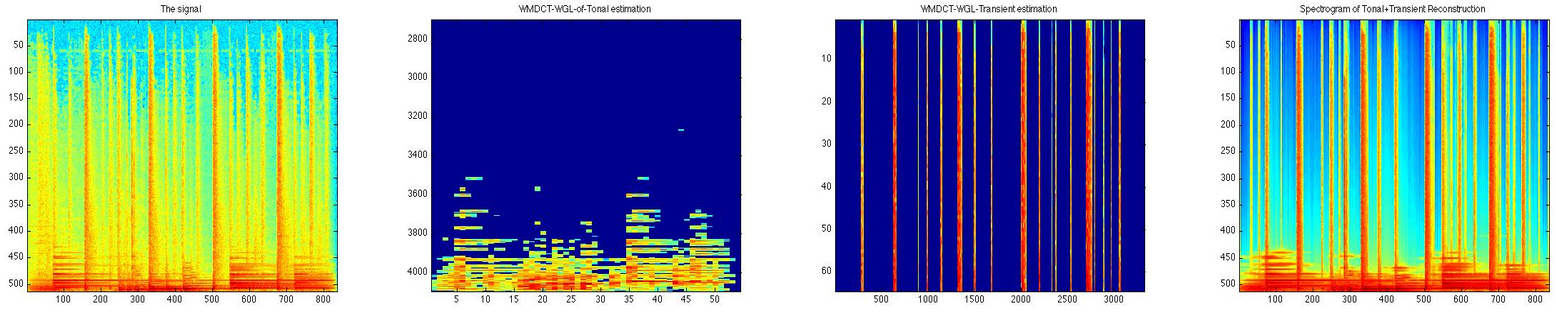
\includegraphics[width=11cm]{./wmdctjazz.png}
		\caption{Audioshrink for tonal/transient separation in jazz music}
		\vspace{-0.5em}
	\end{figure}
	Use 2 WMDCT transforms (wide + narrow window) + Group-LASSO to shrink input signal into significant coefficients in ``time'' and ``frequency'' groups
\end{frame}

\begin{frame}[fragile]
	\frametitle{Audioshrink MATLAB pseudocode}
\begin{figure}[h]
  \centering
  \centering
\begin{minted}[numbersep=\mintednumbersep,linenos,mathescape=true,breaklines,frame=single,escapeinside=||]{text}
|$f = \text{mixed audio}$|
|$F1 = \text{frametight}(\text{frame}(\text{wmdct}, \text{gauss}, \text{winsize}_{h}))\qquad\text{\textbf{WMDCT} }$|
|$F2 = \text{frametight}(\text{frame}(\text{wmdct}, \text{gauss}, \text{winsize}_{p}))$|
|$c1 = \text{franagrouplasso}(F1, f, \lambda_{h}, \text{soft}, \text{freq})$|
|$c2 = \text{franagrouplasso}(F2, f, \lambda_{p}, \text{soft}, \text{time})$|
|$xh = \text{frsyn}(F1, c1)\qquad\qquad\qquad\text{\textbf{Inverse WMDCT} }$|
|$xp = \text{frsyn}(F2, c2)$|
\end{minted}
  \captionof{listing}{WMDCTLasso tonal/transient separation algorithm}
\end{figure}
\textit{franagrouplasso} in LTFAT solves the Group-LASSO regression problem in the time-frequency domain\\
Soft thresholding vs. hard thresholding -- similar to soft/hard masking
\end{frame}

\begin{frame}
	\frametitle{R{\'e}nyi entropy vs. Lasso}
	\begin{itemize}
	\item
		Using Lasso-like methods ($l1,2$ norm in linear least squares regression) assumes that the underlying systems are linear Gaussian, or approximately so\footfullcite{entropy}
	\item
		If the system is not linear-Gaussian, linear least squares regression can lead to suboptimal results
	\item
		R{\'e}nyi entropy, which is an adaptation of Shannon entropy \footfullcite{renyi, shannon1948} is a measure of information in signal processing, and can be used as an optimization target (i.e., loss function) without imposing restrictions on the system being optimized
	\end{itemize}
\end{frame}

\begin{frame}
	\frametitle{Time-Frequency Jigsaw Puzzle}
	\begin{enumerate}
		\item
			Create time-frequency ``super-tiles'' by superimposing a large window + small window Gabor analysis
		\item
			Use R{\'e}nyi entropy to set coefficients to zero where sound has more entropy than random white noise
	\end{enumerate}
	\begin{figure}[ht]
		\vspace{-0.75em}
		\subfloat[TF supertiles]{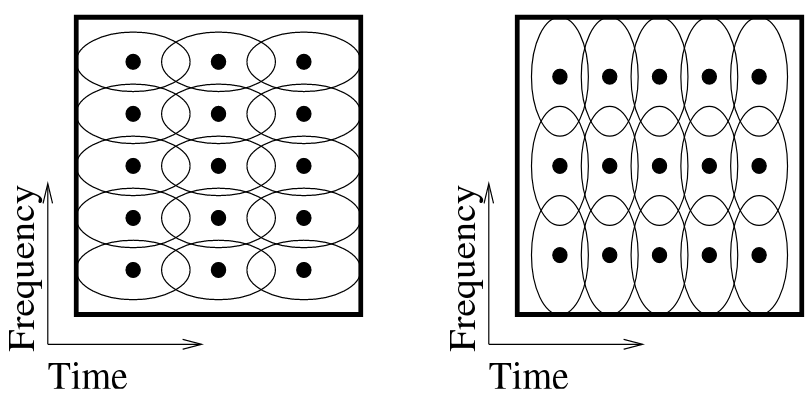
\includegraphics[width=5.25cm]{./tfjigsaw-supertiles.png}}
		\hspace{0.1em}
		\subfloat[Entropy criterion]{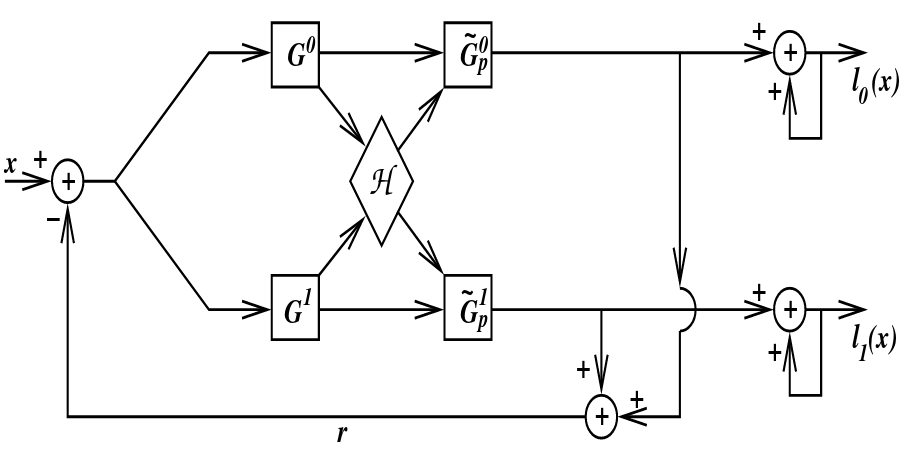
\includegraphics[width=5.25cm]{./tfjigsaw-entropycriterion.png}}
		\caption{TF Jigsaw Puzzle tonal/transient separation\footfullcite{tfjigsaw}}
	\end{figure}
\end{frame}

\note{
	\begin{itemize}
		\item
			i.e. good tonal/good transient
		\item
			high entropy = indicating sound is poorly represented
	\end{itemize}
}


\begin{frame}
	\frametitle{TFJigsaw}
	\begin{figure}[ht]
		\vspace{-1em}
		\subfloat{\makebox[0.4\textwidth]{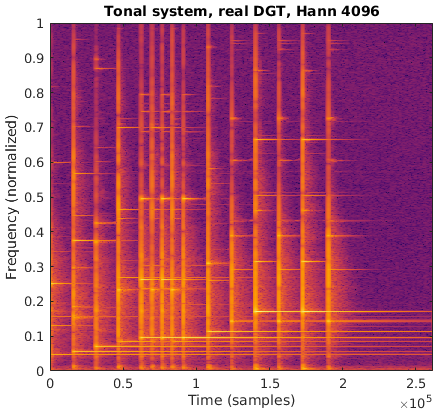
\includegraphics[height=3.5cm]{./glock_dgtreal_tonal.png}}}
		\subfloat{\makebox[0.4\textwidth]{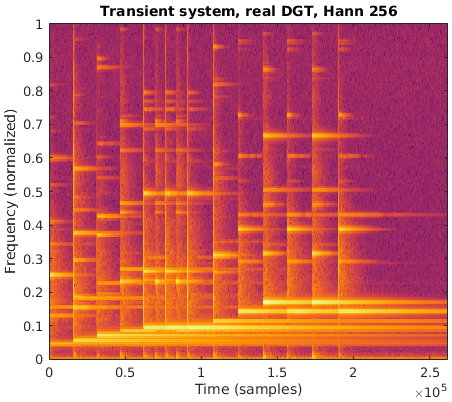
\includegraphics[height=3.5cm]{./glock_dgtreal_transient.png}}}\\
		\vspace{-1em}
		\subfloat{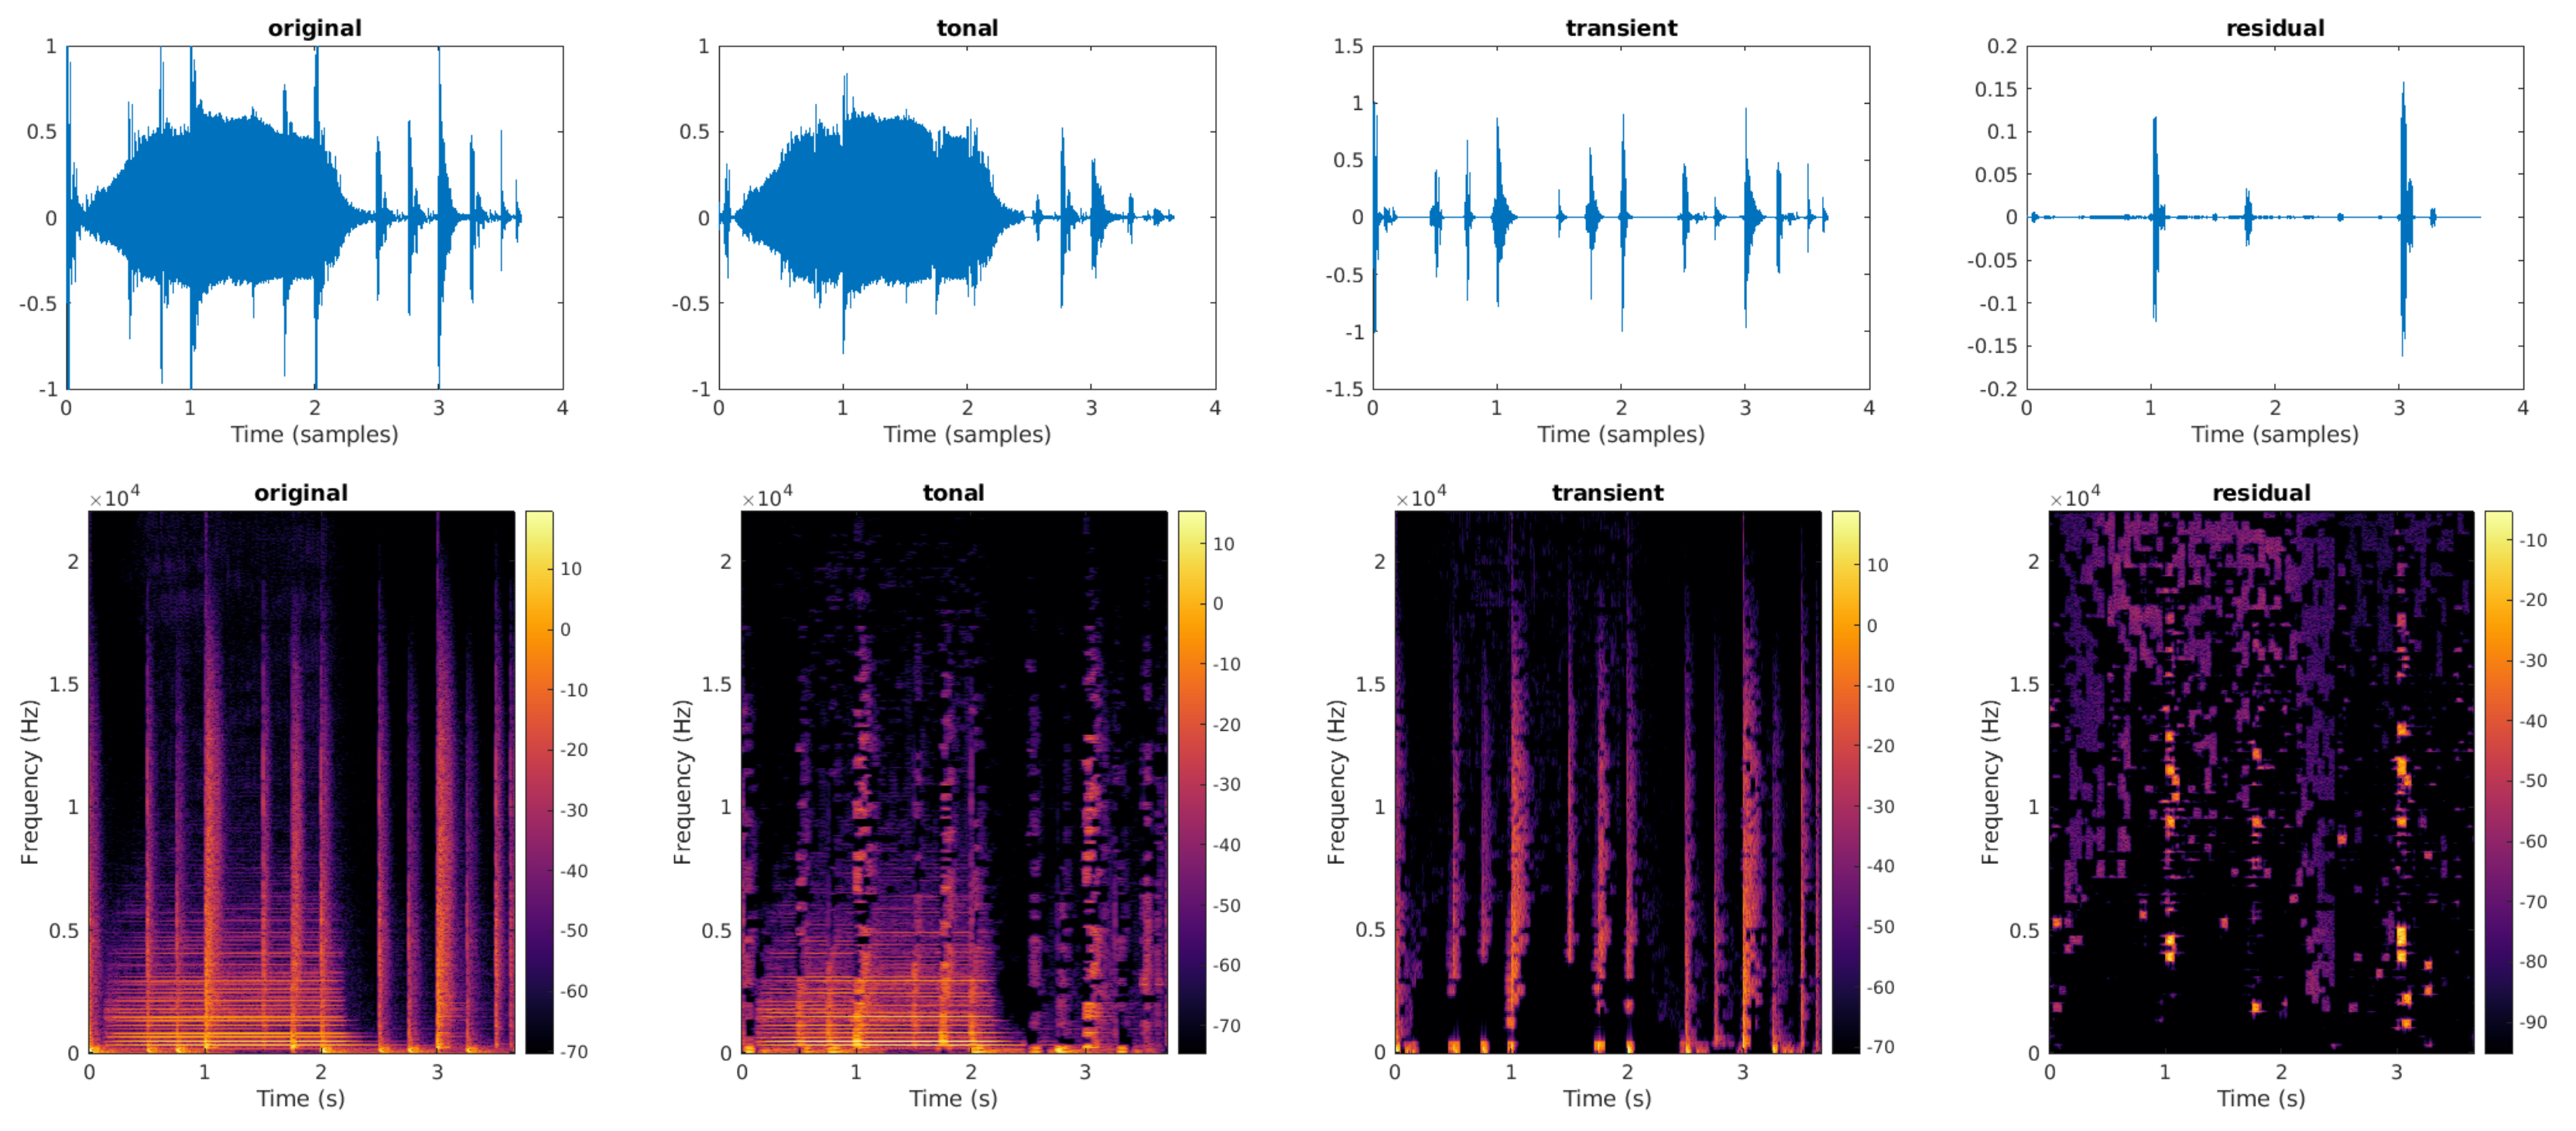
\includegraphics[width=11cm]{./tfjigsaw-sep-example.png}}
		\caption{TF Jigsaw Puzzle tonal/transient separation\footnote{\url{https://ltfat.github.io/doc/sigproc/tfjigsawsep.html}, \url{https://github.com/ltfat/ltfat/blob/master/demos/demo_tfjigsawsep.m}}}
	\end{figure}
\end{frame}

\note{
	\begin{itemize}
		\item
			Hann DGT = stft, basically
	\end{itemize}
}

\begin{frame}[fragile]
	\frametitle{TFJigsaw MATLAB pseudocode}
\begin{figure}[h]
  \centering
\begin{minted}[numbersep=\mintednumbersep,linenos,mathescape=true,breaklines,frame=single,escapeinside=||]{text}
|$f = \text{mixed audio}$|
|$a,M,\text{winsize},b\{1,2\} = \text{Gabor systems 1 and 2 configuration}$|
|$r\{1,2\} = \text{significance level of tonal and transient layer re: white noise ref}$|
|$[\text{ref}1, \text{ref}2] = \text{generate estimate of random white noise entropy within supertile}$|
|$[\text{tau}1, \text{tau}2] = [\text{ref}1 \cdot r1, \text{ref}2 \cdot r2]$|
|$c1 = \text{DGTReal}(f, \text{winsize}1, a1, M1)\qquad\text{\textbf{Discrete Gabor Transform}}$|
|$c2 = \text{DGTReal}(f, \text{winsize}2, a2, M2)$|
|$\text{for all time and frequency supertiles}$|
|$\qquad f\{1,2\} = \text{frequency supertile location, Gabor system 1,2}$|
|$\qquad t\{1,2\} = \text{time supertile location, Gabor system 1,2}$|
|$\qquad [c1, c2] = \text{decision}(c1,c2,f1,f2,t1,t2,\text{tau}1,\text{tau}2)$|
|$\text{endfor}$|
|$f_{\text{tonal}} = \text{IDGTReal}(c1)\qquad\qquad\text{\textbf{Inverse discrete Gabor Transform}}$|
|$f_{\text{transient}} = \text{IDGTReal}(c2)$|
\end{minted}
  \captionof{listing}{TFJigsaw tonal/transient separation algorithm}
\end{figure}
\end{frame}

\begin{frame}
	\frametitle{Evaluation testbench}
	Inspired by SigSep\footnote{\url{https://sigsep.github.io/}}, SISEC (Signal Separation Evaluation Campaign):
	\begin{itemize}
		\item
			BSS\footshortcite{bss} (BSSv4 variant\footnote{\url{https://github.com/sigsep/bsseval}}) and PEASS\footshortcite{peass} (MATLAB toolkit\footnote{\url{http://bass-db.gforge.inria.fr/peass/}}). BSS vs. PEASS?\footshortcite{beassvpeass} BSSv4 is used widely in modern literature,\footshortcite{sigsep2018} but perceptual measures are important! Use PEASS
		\item
			Testing files: MUSDB18-HQ \footshortcite{musdb18-hq}
		\item
			MATLAB/Python testbench using file system + JSON interchanges
		\item
			Open-Unmix\footshortcite{umx} as a reference, open, near-SOTA neural solution
		\item
			Compare different configurations of each algorithm in ``group stages,'' winners move to next stage and may be combined in hybrid algorithms
	\end{itemize}
\end{frame}

\note{
	\begin{itemize}
		\item
			global score omitted. target, interference, artifact
	\end{itemize}
}

\begin{frame}
	\frametitle{HPSS -- PEASS results}
	\begin{figure}[ht]
		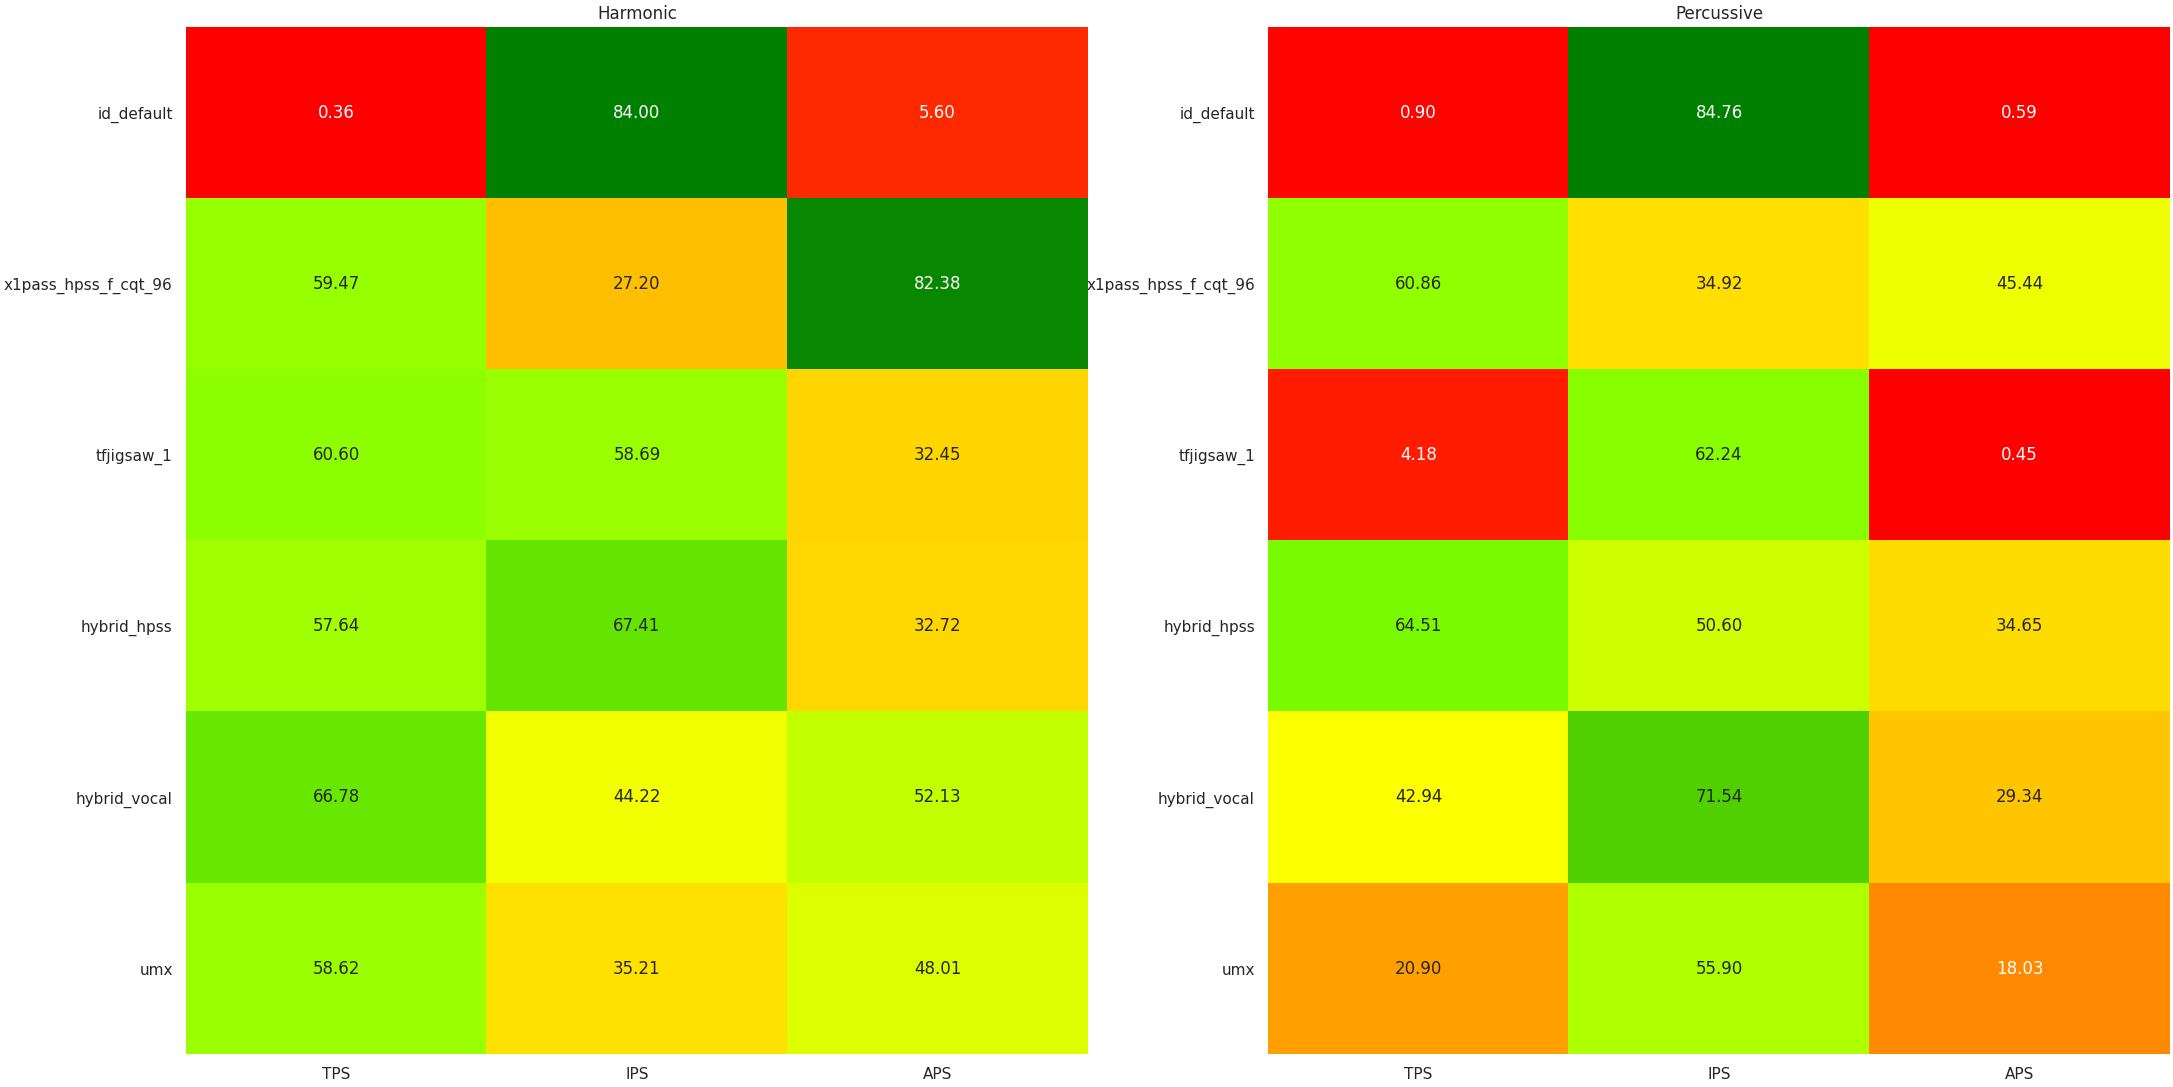
\includegraphics[width=11cm]{../evaluation/heatmaps/Final_HPSS_PEASS_abbrev.png}
		\caption{HPSS algorithms -- final heatmap, PEASS scores}
	\end{figure}
\end{frame}

\begin{frame}
	\frametitle{HPSS -- BSSv4 results}
	\begin{figure}[ht]
		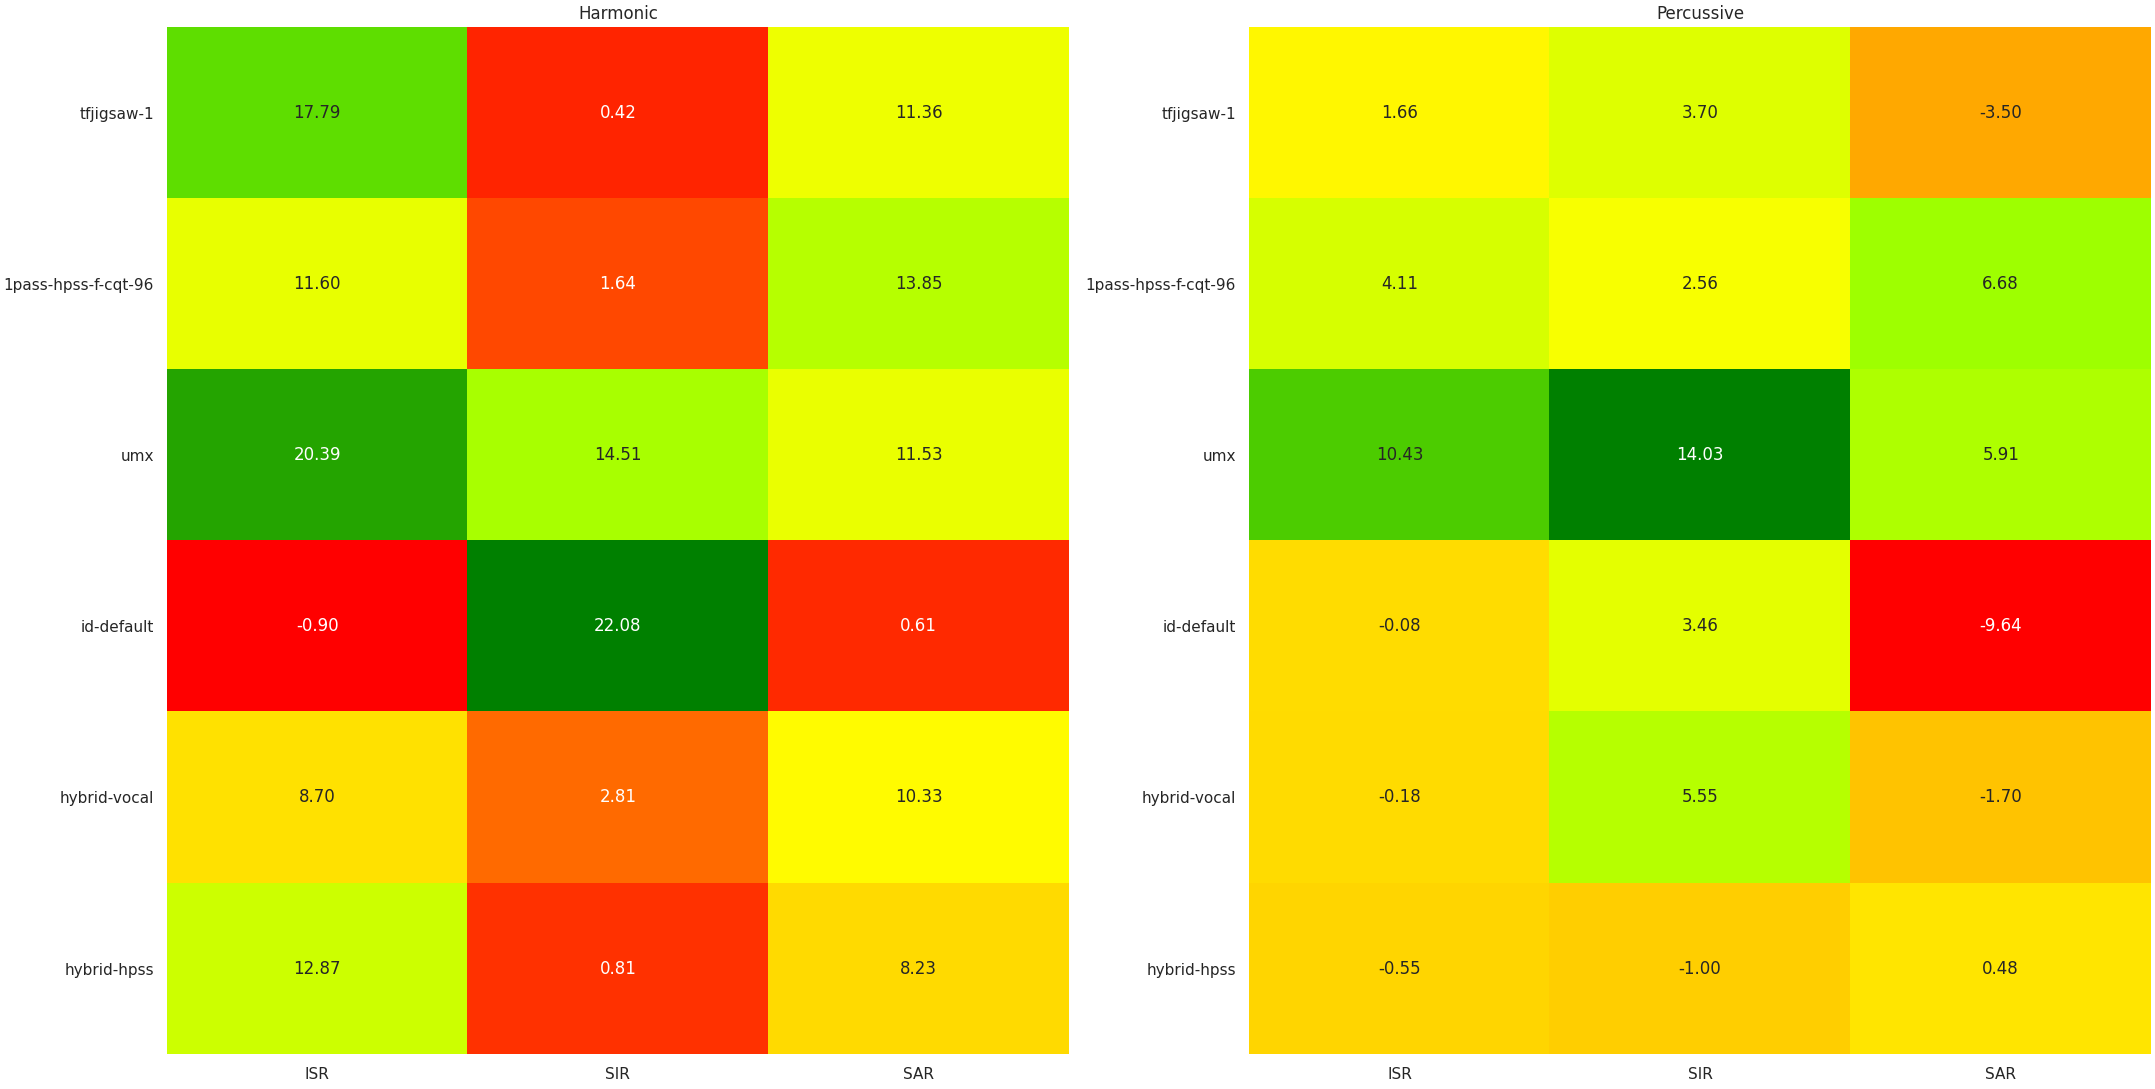
\includegraphics[width=11cm]{../evaluation/heatmaps/Final_HPSS_BSSv4_abbrev.png}
		\caption{HPSS algorithms -- final heatmap, BSSv4 scores}
	\end{figure}
\end{frame}

\begin{frame}
	\frametitle{HPSS + vocal -- PEASS results}
	\begin{figure}[ht]
		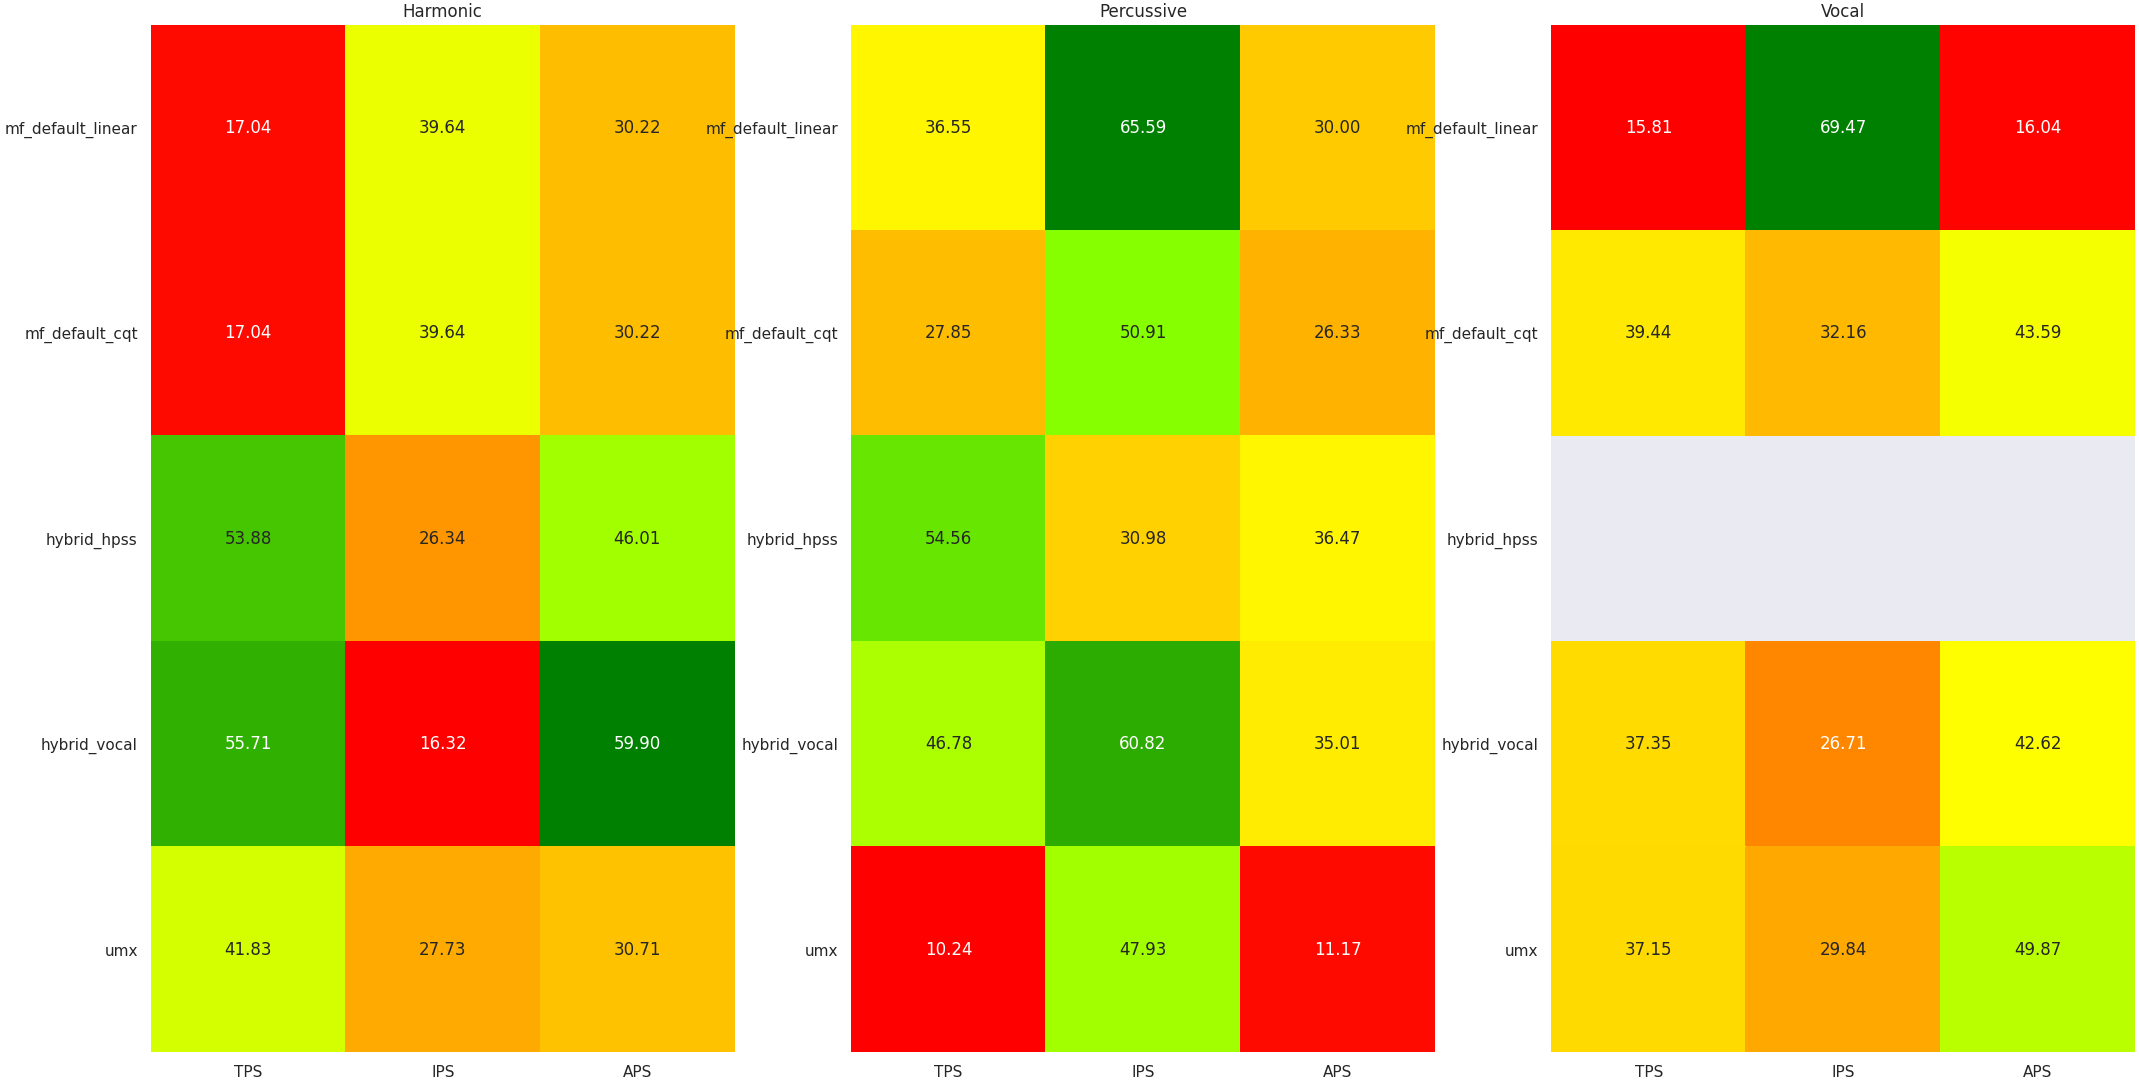
\includegraphics[width=11cm]{../evaluation/heatmaps/Final_Vocal_PEASS_abbrev.png}
		\caption{HPSS + vocal algorithms -- final heatmap, PEASS scores}
	\end{figure}
\end{frame}

\begin{frame}
	\frametitle{HPSS + vocal -- BSSv4 results}
	\begin{figure}[ht]
		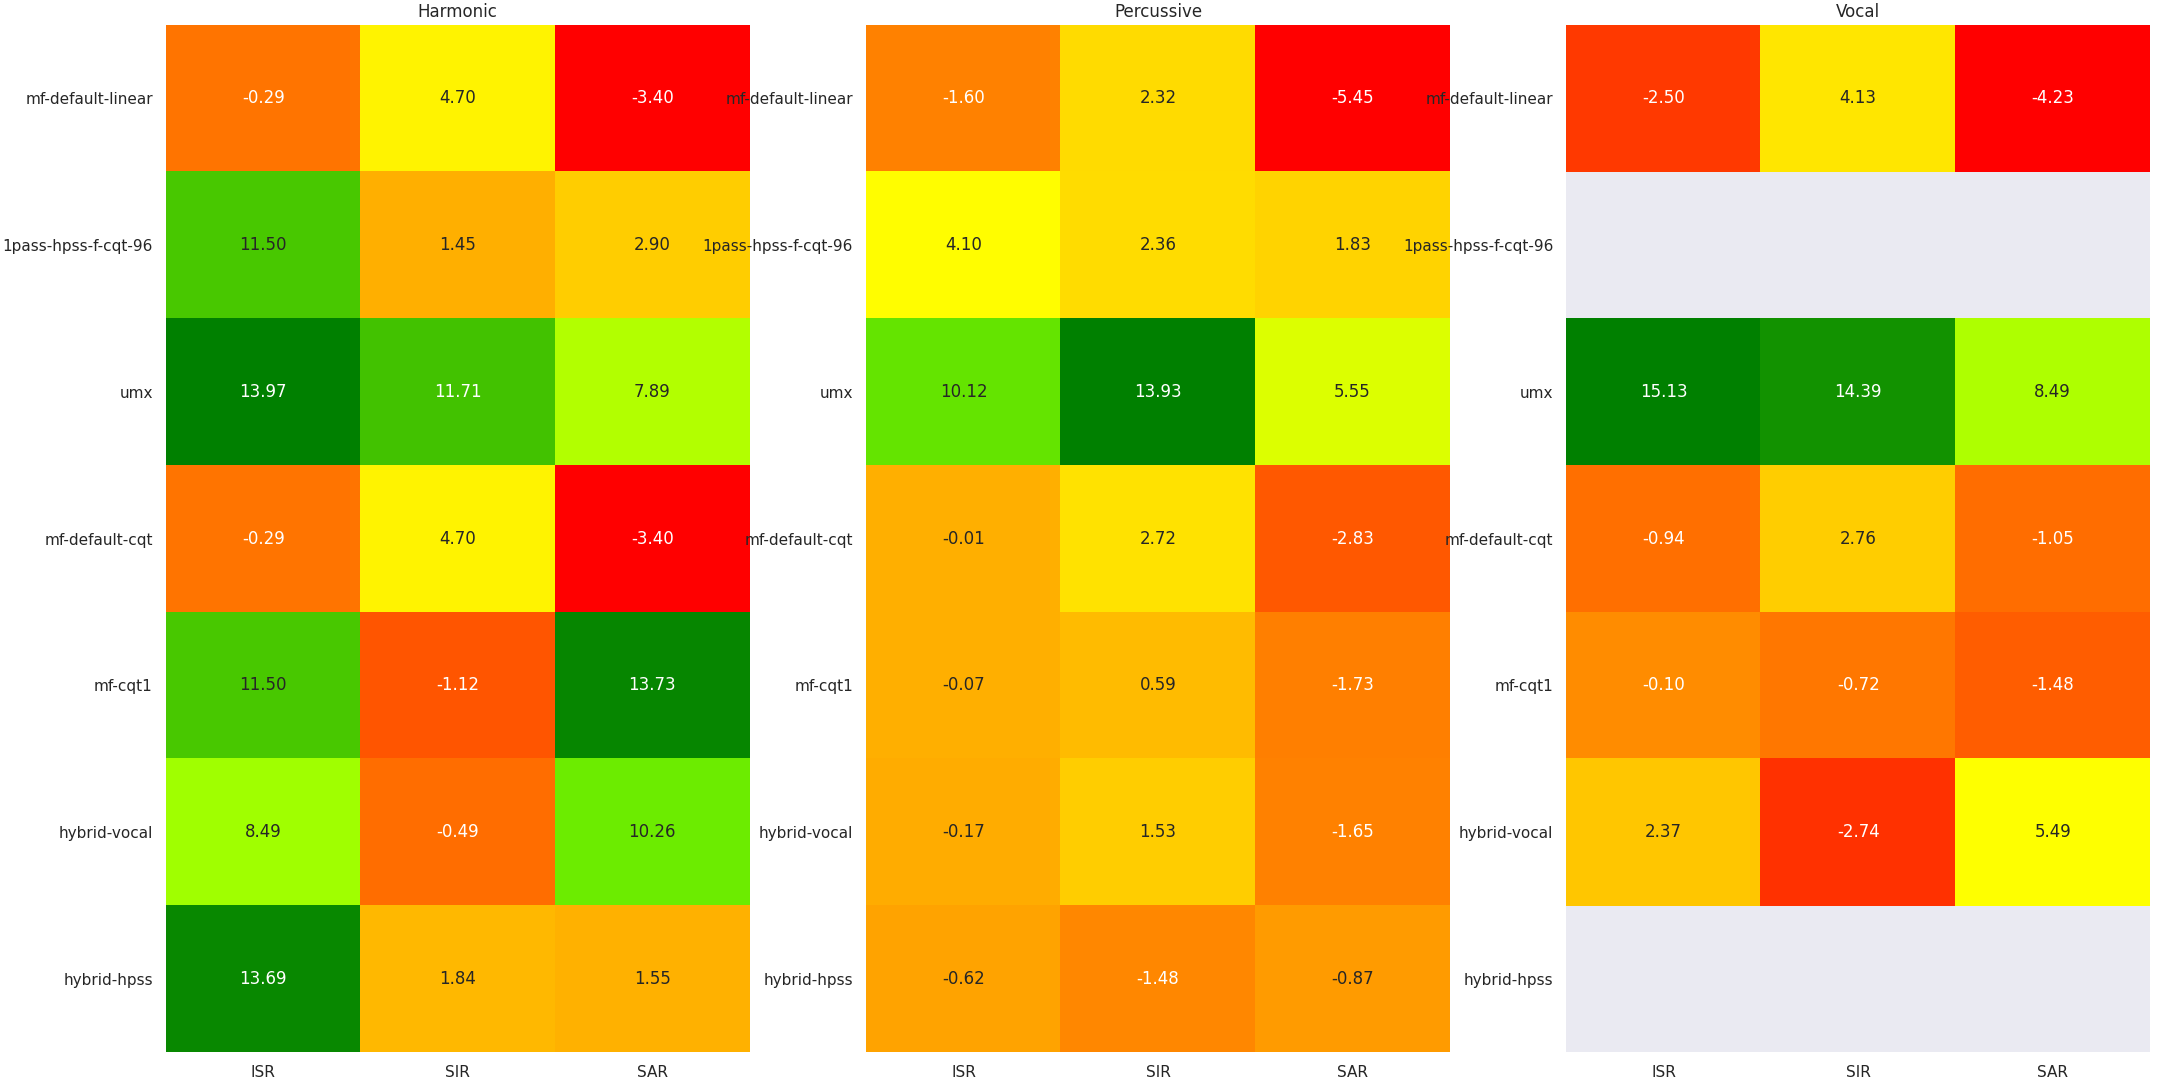
\includegraphics[width=11cm]{../evaluation/heatmaps/Final_Vocal_BSSv4_abbrev.png}
		\caption{HPSS + vocal algorithms -- final heatmap, BSSv4 scores}
	\end{figure}
\end{frame}

\begin{frame}
	\frametitle{Best 1-pass HPSS -- CQT-96, sliCQ median filter}
	Best performing 1-pass offline/anticausal algorithm: CQT with 96 bins-per-octave + median filter + \textbf{soft} mask. Realtime/causal: sliCQ\footfullcite{rtcqt} with 12 bins-per-octave + median filter + \textbf{hard} mask\\
	\begin{figure}[ht]
		\vspace{-0.5em}
		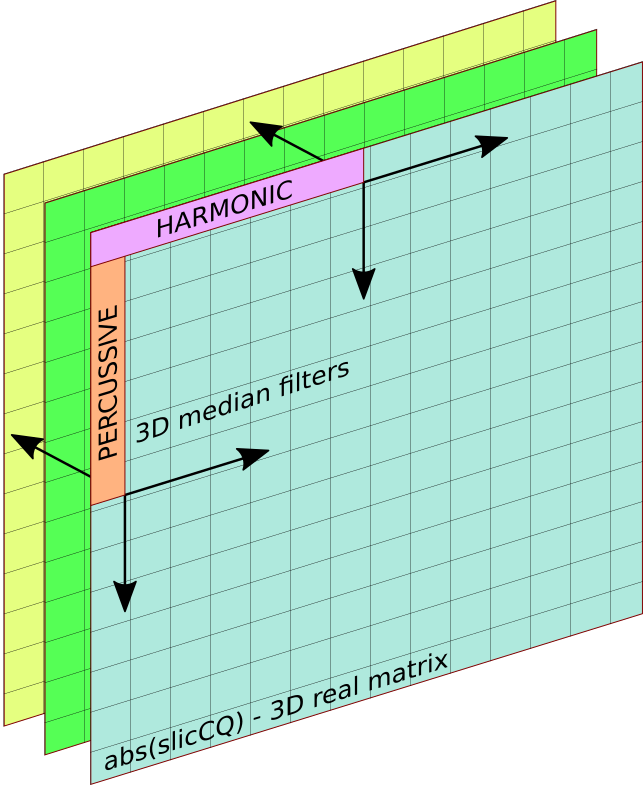
\includegraphics[width=3cm]{./singlemfilt3.png}
		\vspace{-0.75em}
	\end{figure}
	Realtime STFT:\footnote{\url{https://github.com/sevagh/Real-Time-HPSS}} input stream = hop size, $2 \times \text{hop}$ ringbuffer (window). sliCQ transform: input stream = trlen, $4 \times \text{trlen}$ ringbuffer (sllen)
\end{frame}

\note{
	\begin{itemize}
		\item
			3D sliCQ coefficients can be median filtered, analogous to RGB/RGBA images
	\end{itemize}
}


\begin{frame}
	\frametitle{Best 2-pass HPSS -- hybrid}
	Hybrid HPSS: combine TFJigsaw and STFT median filtering
	\begin{figure}[ht]
		\vspace{-0.5em}
		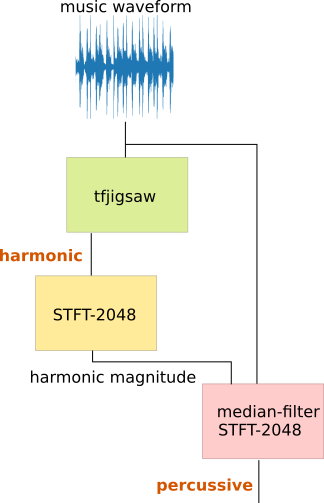
\includegraphics[width=3.5cm]{./hybrid_hpss_block_diagram.png}
		\caption{Block diagram of hybrid HPSS algorithm}
		\vspace{-0.75em}
	\end{figure}
\end{frame}

\begin{frame}
	\adjustbox{valign=c}{{\usebeamerfont{frametitle}\usebeamercolor[fg]{frametitle}Multipass hybrid vocal}}\hfill
	\adjustbox{valign=c}{\makebox[0.5\textwidth]{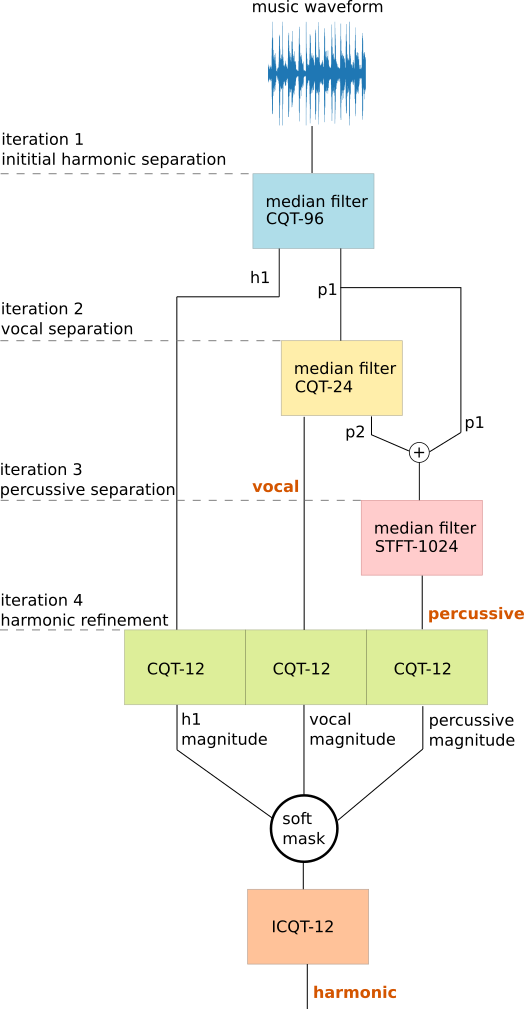
\includegraphics[width=4.5cm]{./hybrid_vocal_block_diagram.png}}}
\end{frame}

\begin{frame}
	\frametitle{HPSS -- audio clips}
	\begin{table}[ht]
	\centering
	\begin{tabular}{lll c c c}
		\hline\hline
		Algorithm & Harmonic & Percussive \\ [0.5ex]
		\hline\hline
		Reference \href{run:./ref_mix.wav}{\faVolumeUp \ mix} & \href{run:./ref_harm.wav}{\faVolumeUp \ h} & \href{run:./ref_perc.wav}{\faVolumeUp \ p} \\ [0.5ex]
		1-pass CQT 96 bins + soft mask \footshortcite{fitzgerald1} & \href{run:./1pass_cqt96_harm.wav}{\faVolumeUp \ h} & \href{run:./1pass_cqt96_perc.wav}{\faVolumeUp \ p} \\ [0.5ex]
		Realtime sliCQ 12 bins + hard mask & \href{run:./rthpss_harm.wav}{\faVolumeUp \ h} & \href{run:./rthpss_perc.wav}{\faVolumeUp \ p} \\ [0.5ex]
		Iterative Driedger\footshortcite{driedger} & \href{run:./driedger_harm.wav}{\faVolumeUp \ h} & \href{run:./driedger_perc.wav}{\faVolumeUp \ p} \\ [0.5ex]
		Hybrid-HPSS & \href{run:./2pass_harm.wav}{\faVolumeUp \ h} & \href{run:./2pass_perc.wav}{\faVolumeUp \ p} \\ [0.5ex]
		UMX & \href{run:./umx_hpss_harm.wav}{\faVolumeUp \ h} & \href{run:./umx_hpss_perc.wav}{\faVolumeUp \ p} \\ [0.5ex]
		\hline
	\end{tabular}
	\end{table}
\end{frame}

\begin{frame}
	\frametitle{HPSS + vocal -- audio clips}
	\begin{table}[ht]
	\centering
	\begin{tabular}{llll c c c c}
		\hline\hline
		Algorithm & Harmonic & Percussive & Vocal \\ [0.5ex]
		\hline\hline
		Reference \href{run:./refv_mix.wav}{\faVolumeUp \ mix} & \href{run:./refv_harm.wav}{\faVolumeUp \ h} & \href{run:./refv_perc.wav}{\faVolumeUp \ p} & \href{run:./refv_vocal.wav}{\faVolumeUp \ v} \\ [0.5ex]
		Iterative Fitzgerald, vocal \footshortcite{fitzgerald2} & \href{run:./mfcqt_harm.wav}{\faVolumeUp \ h} & \href{run:./mfcqt_perc.wav}{\faVolumeUp \ p} & \href{run:./mfcqt_vocal.wav}{\faVolumeUp \ v} \\ [0.5ex]
		Iterative Fitzgerald, percussive & \href{run:./mflinear_harm.wav}{\faVolumeUp \ h} & \href{run:./mflinear_perc.wav}{\faVolumeUp \ p} & \href{run:./mflinear_vocal.wav}{\faVolumeUp \ v} \\ [0.5ex]
		Hybrid-Vocal & \href{run:./2passv_harm.wav}{\faVolumeUp \ h} & \href{run:./2passv_perc.wav}{\faVolumeUp \ p} & \href{run:./2passv_vocal.wav}{\faVolumeUp \ v} \\ [0.5ex]
		UMX & \href{run:./umx_harm.wav}{\faVolumeUp \ h} & \href{run:./umx_perc.wav}{\faVolumeUp \ p} & \href{run:./umx_vocal.wav}{\faVolumeUp \ v} \\ [0.5ex]
		\hline
	\end{tabular}
	\end{table}
\end{frame}

\begin{frame}
	\frametitle{NSGT in STFT-based neural network}
	\begin{figure}
		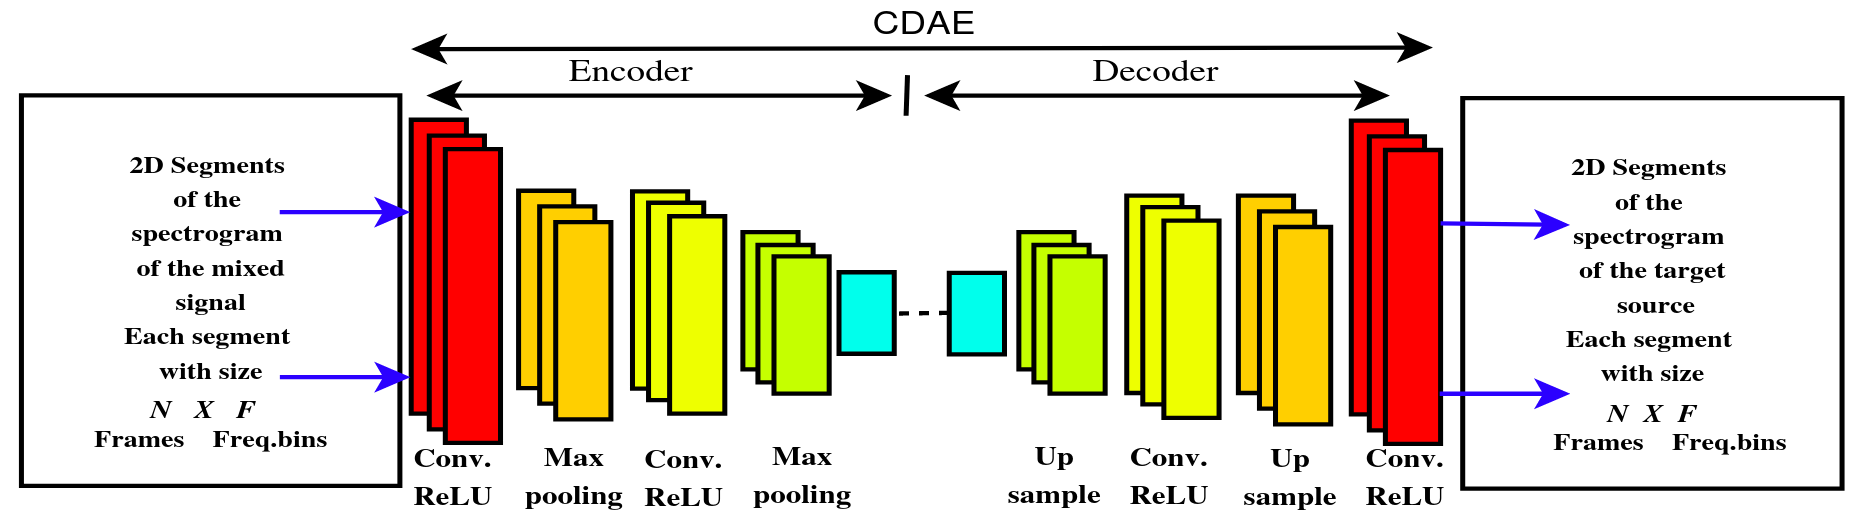
\includegraphics[width=10cm]{./cdae_arch.png}
		\caption{Convolutional denoising autoencoders\footfullcite{cdae}}
	\end{figure}
	Idea: replace STFT spectrogram with NSGT spectrogram. Both MATLAB Wavelet Toolbox CQT (based on NSGT) and reference Python implementation of NSGT (\href{https://github.com/grrrr/nsgt}{https://github.com/grrrr/nsgt}) can produce a rectangular matrix of TF coefficients, solving a common difficulty of using the CQT in spectrogram-based algorithms.
\end{frame}

\begin{frame}
	\frametitle{NSGT-spectrogram neural network}
	\begin{figure}
		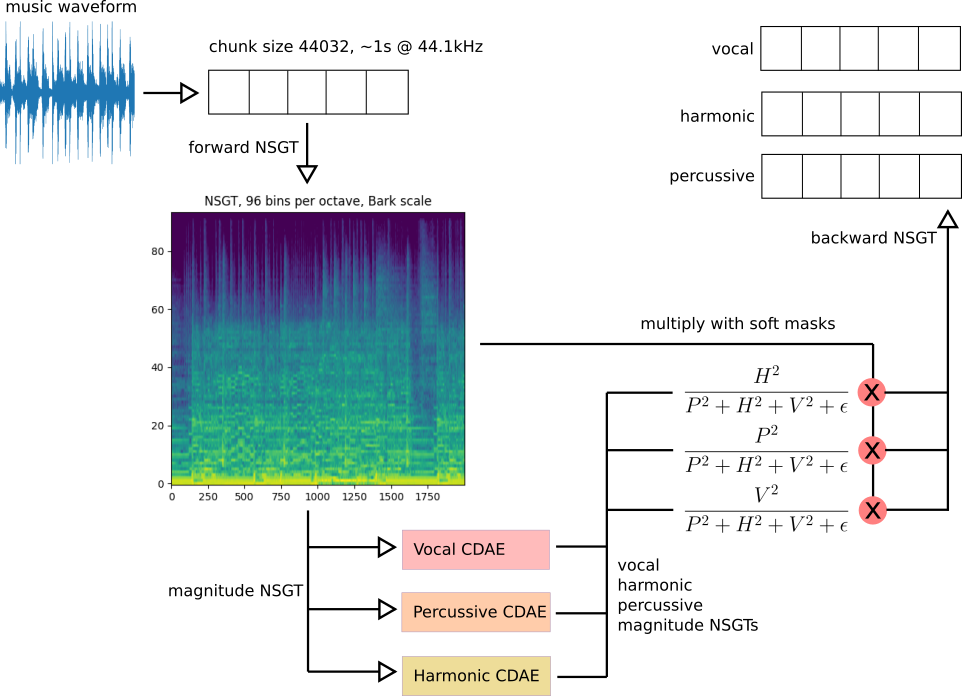
\includegraphics[width=9cm]{./mixin_arch.png}
		\caption{Toy/demo in \href{https://github.com/sevagh/MiXiN}{https://github.com/sevagh/MiXiN}}
	\end{figure}
\end{frame}

\begin{frame}
	\frametitle{Conclusions}
	\begin{itemize}
		\item
			Real-world application of 622 concepts -- sparsity, entropy, overcomplete dictionaries, pursuit
		\item
			Swap STFT for ``better'' TF representations in simple algorithms to improve source separation results
		\item
			Competitive PEASS separation results in hybrid algorithms based on advanced DSP/time-frequency analysis (not so good in BSSv4)
		\item
			Swap STFT for NSGT in a both traditional DSP algorithms, and machine/deep learning networks -- lots of future potential
	\end{itemize}
	501 to 622:
	\begin{table}[ht]
	\centering
	\begin{tabular}{lll c c c}
		\hline\hline
		Algorithm & Harmonic & Percussive \\ [0.5ex]
		\hline\hline
		HPSS (MUMT 501) \href{run:./elmestizo.wav}{\faVolumeUp \ mix} & \href{run:./elmestizo_harm_501.wav}{\faVolumeUp \ h} & \href{run:./elmestizo_perc_501.wav}{\faVolumeUp \ p} \\ [0.5ex]
		MiXiN (MUMT 622) & \href{run:./elmestizo_harm_622.wav}{\faVolumeUp \ h} & \href{run:./elmestizo_perc_622.wav}{\faVolumeUp \ p} \\ [0.5ex]
		\hline
	\end{tabular}
	\end{table}
\end{frame}

\end{document}
